%
% Tesi D.S.I. - modello preso da
% Stanford University PhD thesis style -- modifications to the report style
%
%%%%%%%%%%%%%%%%%%%%%%%%%%%%%%%%%%%%%%%%%%%%%%%%%%%%%%%%%%%%%%%%%%%%%%%%%%%
%                                                                         %
%			TESI DOTTORATO                                                   %
%			______________                                                   %
%                                                                         %
%			AUTORE: Elena Pagani                                             %
%                                                                         %
%			Ultima revisione: 7.X.1998                                       %
%                                                                         %
%%%%%%%%%%%%%%%%%%%%%%%%%%%%%%%%%%%%%%%%%%%%%%%%%%%%%%%%%%%%%%%%%%%%%%%%%%%
%
%
\documentclass[12pt]{report}
   %\renewcommand{\baselinestretch}{1.5}      % interline spacing
%
% \includeonly{}
%
%			PREAMBOLO
%

\usepackage[a4paper]{geometry}
\usepackage{amssymb,amsmath,amsthm}
\usepackage{graphicx}
\usepackage{bm}
\usepackage{url}
\usepackage{wasysym}
\usepackage{hyperref}
\usepackage{epsfig}
\usepackage[italian]{babel}
\usepackage{setspace}
\usepackage{tesi}
\usepackage[sorting=none]{biblatex}
\usepackage{algorithm}
\usepackage{algorithmic}
%\usepackage{algpseudocode}
\usepackage[detect-all]{siunitx} 

\makeatletter
\renewcommand{\ALG@name}{Algoritmo}
\makeatother

% per le accentate
\usepackage[utf8]{inputenc}
%
\newtheorem{myteor}{Teorema}[section]
%
\theoremstyle{definition}
\newtheorem{exmp}{Esempio}[section]

%
\newenvironment{teor}{\begin{myteor}\sl}{\end{myteor}}
\bibliography{references.bib}

%
%
%			TITOLO
%
\makeatletter
\newcommand{\thickhline}{%
    \noalign {\ifnum 0=`}\fi \hrule height 1pt
    \futurelet \reserved@a \@xhline
}
\let\emptyset\varnothing
\newcolumntype{"}{@{\hskip\tabcolsep\vrule width 1pt\hskip\tabcolsep}}
\makeatother
\begin{document}
\title{Rilevazione di fake news\\ basata sull'induzione di insiemi fuzzy}
\author{Giovanni LAGANÀ}
\dept{Corso di Laurea Magistrale in Informatica}
\anno{2019-2020}
\matricola{928792}
\relatore{Prof. Dario MALCHIODI}
\correlatore{Prof. Alfio FERRARA}
%
%        \submitdate{month year in which submitted to GPO}
%		- date LaTeX'd if omitted
%	\copyrightyear{year degree conferred (next year if submitted in Dec.)}
%		- year LaTeX'd (or next year, in December) if omitted
%	\copyrighttrue or \copyrightfalse
%		- produce or don't produce a copyright page (false by default)
%	\figurespagetrue or \figurespagefalse
%		- produce or don't produce a List of Figures page
%		  (false by default)
%	\tablespagetrue or \tablespagefalse
%		- produce or don't produce a List of Tables page
%		  (false by default)
%
%			DEDICA
%
\beforepreface
        {\hfill \Large {\sl \begin{flushright} Dedica da inserire.         
\end{flushright}         }}
%
%			PREFAZIONE
%
%\prefacesection{Prefazione}
%hkjafgyruet.
%
%%
%%
%%			ORGANIZZAZIONE
%\section*{Organizzazione della tesi}
%\label{organizzazione}
%La tesi \`e organizzata come segue:
%\begin{itemize}
%\item nel Capitolo 1 ....
%\end{itemize}
%
\afterpreface

%
%
%			CAPITOLO 1: 

\chapter*{Introduzione}
\addcontentsline{toc}{chapter}{Introduzione} \markboth{Introduzione}{} 
\onehalfspacing

Prova per citare tutti i libri
\cite{1,2,3,4,5,6,7,8,9,10,11,12,13,14,15,16,17,18,19,20,21,22}


\chapter{Stato dell'arte}
\label{Capitolo 1}
\onehalfspacing

Il capitolo che apre questa tesi è inerente allo stato dell'arte e si compone come segue: il Paragrafo \ref{fakenews} descrive il problema delle fake news, menzionando la disciplina del fact-checking; il Paragrafo \ref{nlp} riporta le tecniche di elaborazione del linguaggio naturale, soffermandosi sulla gestione del rumore per la fase di preprocessing, sulla rielaborazione del testo e sull'embedding per convertire tale testo in un dato di tipo numerico. 
Il Paragrafo \ref{insiemifuzzy} presenta il concetto degli insiemi fuzzy e fornisce una motivazione del perché essi siano uno strumento adeguato per il problema delle fake news.
Infine, il Paragrafo \ref{induzione} porta alla luce i principali componenti del processo di induzione considerato.

\section{Fake news} \label{fakenews}
L'avvento dei news media e dei social media ha portato a una proliferazione e a un consumo crescenti di notizie.
In generale, la circolazione di notizie su questi canali ha fatto sì che aumentassero esponenzialmente le cosiddette \textit{fake news}.
\\
Per fake news si intendono quelle notizie riportanti fatti che volutamente non corrispondono alla realtà.
In questo senso, si evidenzia la necessità di riconoscere e combattere questo fenomeno con l'obiettivo di contrastare il fomentare dell'odio, un'arma che al giorno d'oggi può essere usata come carburante di diffamazione, lucro, terrorismo e xenofobia.
\\
Il problema di questo tipo di notizie è che possono mischiarsi con tutte le altre, portando il lettore a confondere un fatto realmente accaduto con uno volutamente modificato a proprio vantaggio per un secondo fine.
Inoltre, esiste un'intrinseca difficoltà nel valutare la veridicità di una notizia sia per il problema di attingere a fonti attendibili, sia per la natura stessa del testo scritto.

\subsection{Fact-checking} \label{factchecking}
Al di là di quale sia il secondo fine di chi diffonde fake news, il nemico numero uno del giornalismo è la disinformazione.
Per questo motivo un lavoro da sempre svolto da giornalisti, e non, è quello del \textit{fact-checking}: si tratta di una serie di attività mirate alla verifica accurata e puntuale delle fonti.
Secondo questo criterio, la verifica delle sorgenti di informazione avrebbe il vantaggio di validare i fatti, non lasciando spazio ad avvenimenti non confermati da fonti autorevoli.
Questo approccio, però, presenta delle criticità, ad esempio l'assunzione che una fake news non abbia fonti: esistono notizie che, pur attenendosi alle fonti, possono esaltare aspetti apparentemente secondari o di dettaglio che, se esasperati, possono alterare la narrazione di un fatto, fino a sconvolgerla.
\\
Un altro aspetto è che non è così semplice stabilire con certezza quando una fonte sia autorevole e quando no; inoltre, è opinabile assumere a priori che una fonte considerata autorevole non commetta mai a sua volta errori di questo tipo.
\\
Uno dei problemi maggiori, oltre al fatto che la verifica della veridicità di una notizia richieda del tempo, è che la smentita non finisce mai per avere la stessa risonanza e visibilità della notizia falsa. Questo amplifica l'esigenza di trovare un metodo per prevenire il problema, piuttosto che risolverlo a posteriori.
\\
La necessità di arginare questo fenomeno ha spinto i media, soprattutto tradizionali, a impegnarsi in un costante lavoro di fact-checking, lungo, impegnativo e reso ancora più difficile dal fatto che spesso le varie realtà agiscono in maniera autonoma.
\\
Ci si chiede, quindi, se il progresso in ambito informatico possa contribuire ad arginare il problema in maniera efficace.
\\
In letteratura sono stati fatti vari studi per la cosiddetta automazione del fact-checking \cite{5, 6, 8, 9, 10, 11}; inoltre, in \cite{15, 16, 21} sono stati proposti approcci che, principalmente, si suddividono nelle categorie focalizzate rispettivamente sui metodi \textit{content-based} e \textit{context-based}.
Mentre il primo approccio lavora sul contenuto testuale a livello sintattico, il secondo tenta di estrapolarne il contesto, lavorando a livello semantico.

\section{Elaborazione del linguaggio naturale} \label{nlp}
L'automazione dell'analisi lessicale fa parte dell'ampia branca dell'Informatica che prende il nome di NLP, \textit{Natural Language Processing}, che tra le sue varie declinazioni presenta degli interessanti strumenti per poter estrarre delle feature a partire da dati testuali come le notizie.


\subsection{Tecniche di gestione del rumore} \label{clean}
Come nella stragrande maggioranza dei dataset, anche in quelli testuali è presente del rumore, sia a ``basso livello'' nel contenuto dell'informazione, sia ad ``alto livello'' nella forma dei dati che si sta utilizzando.
\\
Possono essere molte le motivazioni che portano un dataset a presentare errori, anomalie o rumore al suo interno: 
nel caso di osservazioni raccolte manualmente può verificarsi una componente di errore umano; dualmente, dataset generati automaticamente (ad esempio tramite dati raccolti da sensori) possono presentare delle anomalie e produrre risultati imprevisti.
\\
Nel caso dei dati trattati in questa tesi, inoltre, si ha a che fare con informazioni provenienti dal Web, dunque esiste una maggior probabilità di incontrare osservazioni di natura digitale ricavate da pagine HTML o, addirittura, influenzate dal tipo di codifica scelto per rappresentare caratteri speciali.
In tal senso esistono numerose tecniche per gestire il rumore e, seguendo la distinzione fatta all'inizio di questo paragrafo, è possibile elencare alcune di esse.
\\
\\
Ad \textit{alto livello} si gestisce la presenza di:
\begin{itemize}
    \item valori mancanti,
    \item osservazioni duplicate,
    \item osservazioni vuote,
\end{itemize}

mentre a \textit{basso livello}, tipicamente, si riscontrano:
\begin{itemize}
    \item caratteri speciali,
    \item URL,
    \item parole contenenti numeri,
    \item punteggiatura,
\end{itemize}

e altri numerosi casi che potrebbero essere aggiunti a questo elenco.
\subsection{Tecniche per rielaborare il testo}
Esistono delle procedure per riadattare il testo in una forma più conveniente per sua la successiva elaborazione da parte di algoritmi di Machine Learning.
\\
Vari studi nel campo dell'Information Retrieval \cite{22}, infatti, hanno dimostrato che tecniche come lo \textit{stemming}, la \textit{lemmatizzazione} e la rimozione delle cosiddette \textit{stop word} possono migliorare sensibilmente i risultati ottenuti da tali modelli.

\paragraph{Stemming} Lo stemming consiste nell'individuare e rimuovere il prefisso e il suffisso delle parole, in modo da ricavarne la radice, ne viene mostrato un esempio in Tabella \ref{stemming}.
\begin{table}[!h]
\centering
 \begin{tabular}{|c|c|c|} 
 \hline 
 \textbf{Forma} & \textbf{Suffisso} & \textbf{Radice}
\\ [0.5ex] 
\hline
pront\textbf{o} & \textbf{-o} & \textbf{pront} \\
pronunc\textbf{erà} & \textbf{-erà} & \textbf{pronunc} \\
pronunc\textbf{ia} & \textbf{-ia} & \textbf{pronunc} \\
 \hline
\end{tabular}
\caption{Esempio di stemming.}
\label{stemming}
\end{table}

\paragraph{Lemmatizzazione} La lemmatizzazione prende in considerazione l'analisi morfologica delle parole ricorrendo a dettagliati dizionari che l'algoritmo utilizza per ottenere il lemma associato.
Un esempio di questa tecnica viene mostrato in Tabella \ref{lemmatization}.
\begin{table}[!h]
\centering
 \begin{tabular}{|c|c|c|} 
 \hline 
 \textbf{Forma} & \textbf{Informazione morfologica} & \textbf{Lemma}
\\ [0.5ex] 
\hline
ragazze & femminile plurale di \textbf{ragazzo} & \textbf{ragazzo} \\
studia & terza persona singolare, presente del verbo \textbf{studiare} & \textbf{studiare} \\
studiando & gerundio del verbo \textbf{studiare} & \textbf{studiare} \\
 \hline
\end{tabular}
\caption{Esempio di lemmatizzazione.}
\label{lemmatization}
\end{table}

\paragraph{Rimozione delle stop word}
Gli articoli, le proposizioni, le congiunzioni o gli aggettivi sono esempi tipici di stop word. Queste parole hanno solitamente un'alta frequenza nei documenti ma non aggiungono alcun valore semantico al testo, in quanto sono tipicamente necessarie per la grammatica del linguaggio; pertanto, rimuoverle è una soluzione che viene spesso adottata per ridurre il carico computazionale dell'algoritmo che processa il testo.
\\
\\
Naturalmente, le considerazioni fatte per queste tre tecniche valgono per qualsiasi idioma; tipicamente, le librerie che le implementano presentano delle interfacce per specificare con quale lingua si intende lavorare in maniera da ricorrere a opportuni dizionari.

\subsection{Tecniche di embedding} \label{embedding}
Gli algoritmi di Machine Learning vengono eseguiti per generare dei modelli che sono in grado di fare delle predizioni. Tuttavia, sia i modelli che gli algoritmi in questione necessitano di un input numerico; dal momento che l'obiettivo di questa tesi è trattare le notizie, cioè un dato tipo di testuale, è fondamentale ricorrere a delle tecniche per produrre una rappresentazione quantitativa delle notizie.
In questo senso, le tecniche di embedding intervengono proprio per trasformare il dato testuale in dato numerico.
Concretamente, questo equivale a trovare una rappresentazione numerica del testo, estraendo delle feature.
\\
Due famose tecniche di embedding sono Word2Vec e Doc2Vec, il cui meccanismo viene illustrato nei paragrafi che seguono.
\subsubsection{Word2Vec} \label{w2v}
Word2Vec è un algoritmo che ha l'obiettivo di trasformare le parole in vettori numerici all'interno di uno spazio  di dimensione prefissata \cite{3}.
Un corpus è composto da documenti e ogni documento è composto da parole; ciascuna di queste parole, tramite Word2Vec, viene trasformata in un vettore di lunghezza $h$, dove $h$ indica il numero di feature numeriche che vengono considerate. 
\\
Word2Vec si basa sull'utilizzo di reti neurali \cite{3} ed è principalmente implementato tramite due modelli: Skip-Gram e CBOW (Continuous Bag of Words) che vengono descritti qui di seguito.
\\
Per entrambi i modelli l'input è un corpus di documenti, le cui parole vengono distinte in \textit{token}; ciascun token viene codificato con una rappresentazione one-hot\footnote{La codifica one-hot è un processo che viene applicato ai dati categoriali per convertirli in una rappresentazione vettoriale binaria da utilizzare negli algoritmi di apprendimento automatico. In questo caso i dati categoriali sono le parole e ciascuna può essere rappresentata come il vettore binario di tutti i termini presenti nel documento. Se $n$ è il numero di parole, allora il vettore sarà composto da $n-1$ zeri e da un uno, a indicare quale token venga effettivamente rappresentato}.
\\
Per differenziare le due soluzioni, è necessario introdurre il concetto di contesto, poiché Skip-Gram e CBOW lavorano in due direzioni speculari:
mentre la prima si pone l'obiettivo di predire le parole di contesto a partire dal token corrente, la seconda ha lo scopo di predire il token corrente da una finestra di parole di contesto.
\\
Quando una parola $P$ appare in un testo, il suo contesto è quel set di parole che gli appaiono accanto, data una finestra di analisi precedentemente impostata. I molteplici contesti in cui la parola $P$ viene utilizzata servono a costruire una rappresentazione dell’uso di $P$.
\\
Ogni parola viene associata a un vettore denso, ossia una scala di valori numerici vettoriali, che a sua volta viene messo in associazione con vettori di parole che appaiono in contesti simili, costruendo quelli che vengono definiti \textit{word vectors}.

\paragraph{Skip-Gram}
Si stabilisce una finestra di dimensione $m$ e si scorre ogni token andando a vedere i termini in prossimità, osservando quelli all'interno del raggio $m$.
\\
\begin{figure}
    \centering
    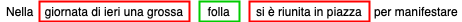
\includegraphics[scale = 0.7]{images/skip-gram.png}
    \caption{Esempio di Skip Gram: in verde il token corrente, in rosso la finestra di contesto grande 5 token.}
    \label{skipgram}
\end{figure}
\\
Per esempio, come illustrato in Figura \ref{skipgram}, se \textit{folla} è il token corrente, con $m = 5$ il confronto avviene con \{\textit{giornata}, \textit{di}, \textit{ieri}, \textit{una}, \textit{grossa}, \textit{si}, \textit{è}, \textit{riunita}, \textit{in}, \textit{piazza}\}.
\\
L'idea è quella di cercare di costruire il mapping tra $X$, i token correnti (es: \textit{folla}), e $y$, i token estratti dalla finestra di contesto (es: \textit{piazza}).
\\
Seguendo la notazione tipica di un problema di apprendimento supervisionato, i token presi dalla finestra di contesto sono la variabile target da predire, apprendendo il tipo di relazione che sussiste tra  $X$ e $y$.
Per farlo, come accennato in precedenza, si utilizza una rete neurale, passando la rappresentazione one-hot del dato a un'unità softmax\footnote{Softmax è una possibile funzione di attivazione dello strato di output della rete neurale. In realtà, vale la pena menzionare altre due varianti di criteri di addestramento applicabili, come Negative sampling e Hierarchical Softmax, con diverse implicazioni riguardo efficienza e onere computazionale.}, una funzione che permette di calcolare la distribuzione di probabilità dei valori possibili nella classificazione multi-classe. Come previsto per le reti neurali, si minimizza una funzione di perdita che, in questo caso, è l'entropia incrociata, utilizzando il metodo del gradiente discendente. 

\paragraph{CBOW}
Dualmente a Skip-Gram, CBOW si occupa di predire il token corrente a partire dalla finestra di contesto.
\\
Come mostrato in Figura \ref{cbow}, si predice con quale probabilità si ottenga il token \textit{folla} a partire dalla finestra \{\textit{giornata}, \textit{di}, \textit{ieri}, \textit{una}, \textit{grossa}, \textit{si}, \textit{è}, \textit{riunita}, \textit{in}, \textit{piazza}\}.
\\
\begin{figure}
    \centering
    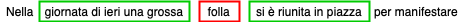
\includegraphics[scale = 0.7]{images/cbow.png}
    \caption{Esempio di CBOW: in rosso il token corrente, in verde la finestra di contesto grande 5 token.}
    \label{cbow}
\end{figure}
\\
Anche in questo caso viene addestrata una rete neurale utilizzando il metodo del gradiente discendente per ottenere l'embedding.
\\
\\
In generale, data la natura di queste tecniche, per ottenere una rappresentazione compatta dell'intero documento si rende necessario l'utilizzo di una tecnica di aggregazione.
In questa fase ogni documento $i$ è formato da $n_i$ parole ed ogni parola è rappresentata da un vettore di $h$ feature. L'aggregazione interviene per comprimere ciascuno di questi vettori in un valore che sia rappresentativo della corrispondente parola, ottenendo così un vettore per l'intero documento.
\\
Così come in tante altre applicazioni dell'Informatica, i metodi di aggregazione sono molteplici, ad esempio la media aritmetica, la mediana, l'aggregazione del kernel di Fisher \cite{19}.
\\
Fare la media tra vettori significa poter agire su due dimensioni, la prima prevede di sommare prima gli elementi di ciascun vettore e poi dividere per il numero di elementi, ottenendo $n_i$ valori medi. In realtà, questa soluzione è scomoda per la successiva elaborazione dei dati, dal momento che ogni documento $i$ può avere un numero variabile di parole e dunque si otterrebbero vettori di lunghezza diversa per il corpus finale.
\\
La soluzione utilizzata, invece, si applica sommando i primi elementi di tutti i vettori, i secondi, i terzi e così via, per poi dividere per il numero di parole. Così facendo si preserva la rappresentazione tramite feature, perchè si ottiene per ogni documento un vettore lungo $h$; un discorso analogo vale per la mediana.
\\
L'aggregazione del kernel di Fisher, invece, propone una rappresentazione che si basa su quanto il vettore osservato si discosti dal modello generativo GMM (Gaussian Mixture Model). Tale discostamento è una misura di distanza che viene calcolata tramite il gradiente di una funzione di verosomiglianza; i vettori ottenuti prendono il nome di \textit{Fisher vectors}.

\subsubsection{Doc2Vec} \label{d2v}
Doc2Vec nasce come evoluzione di Word2Vec: in questo caso, anziché lavorare a livello di ogni singola parola, si determina direttamente una rappresentazione vettoriale per l'intero documento \cite{24}.
Questo comporta chiaramente il raggiungimento del risultato senza ricorrere a un metodo di aggregazione dei valori.
\\
Conosciuto anche come \textit{Paragraph Vector}, Doc2Vec si articola in due principali implementazioni: PV-DM (Distributed Memory) e DBOW (Distributed Bag of Words).

\paragraph{PV-DM} 
Come per Word2Vec, il task che viene fatto ripetutamente è quello di predire la parola successiva nella frase. I vettori delle parole e i vettori dei paragrafi sono chiamati a contribuire a tale predizione.
\\
Ogni paragrafo viene mappato in un vettore, rappresentato da una colonna nella matrice $D$, così come il vettore di ogni parola è rappresentato da una colonna della matrice $P$ (Figura \ref{pvdm}). I vettori menzionati vengono mediati o concatenati e, a loro volta, essi vengono passati alla rete neurale per prevedere la parola centrale.
\\
La rappresentazione del paragrafo è ciò che effettivamente distingue questa tecnica da Word2Vec in quanto, pur agendo come un'altra parola, svolge il ruolo di memoria per ricordare cosa manca al contesto corrente; da qui, il nome \textit{Distributed Memory}.
\\
\begin{figure}
    \centering
    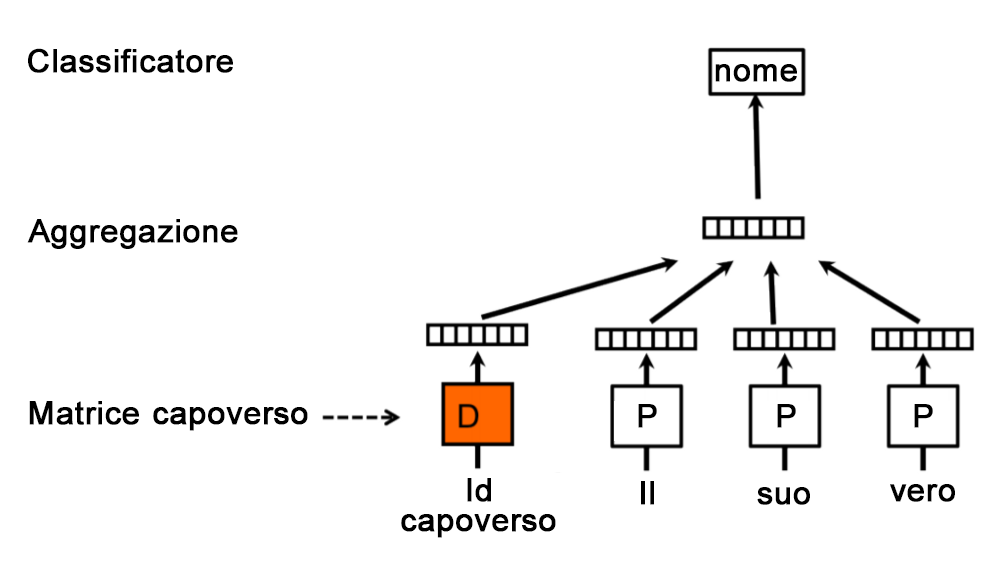
\includegraphics[scale = 0.3]{images/pvdm.png}
    \caption{Architettura in PV-DM (D è la matrice dei documenti e P la matrice delle parole).}
    \label{pvdm}
\end{figure}
\\
La matrice del paragrafo ha, infatti, gli embedding per i paragrafi ``visti'', allo stesso modo in cui i modelli Word2Vec apprendono gli embedding per le parole. Per i paragrafi non visualizzati, invece, il modello viene nuovamente eseguito più volte attraverso la discesa del gradiente per generare un vettore del documento. 

\paragraph{DBOW}
L'architettura DBOW non utilizza le parole di contesto ma effettua la predizione direttamente dalle parole campionate dal paragrafo.
\\
\begin{figure}
    \centering
    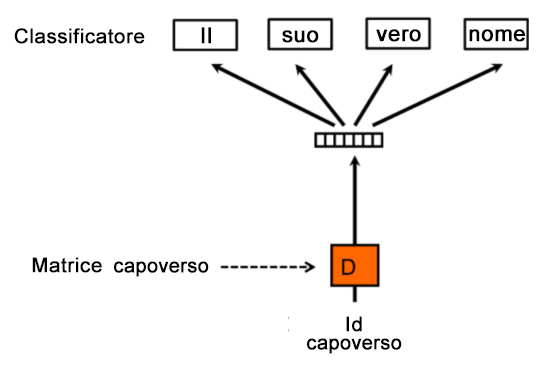
\includegraphics[scale = 0.45]{images/dbow.png}
    \caption{Architettura in DBOW.}
    \label{dbow}
\end{figure}
\\
Ne risulta un'architettura (Figura \ref{dbow}) simile a PV-DM ma con il primo livello costituito unicamente dalla matrice dei paragrafi.

\section{Insiemi fuzzy} \label{insiemifuzzy}
Dal momento che questa tesi si pone l'obiettivo di analizzare le notizie e, nello specifico, di valutare un criterio per individuare quelle fake, è importante introdurre il concetto degli \textit{insiemi fuzzy}.
\\
Diversamente da quanto accade per gli insiemi classici, in cui l'appartenenza  è un concetto binario che viene espresso da un valore di verità, negli insiemi fuzzy esso viene quantificato da un valore continuo tra 0 e 1.
Tale valore prende diversi nomi, come \textit{grado di verità} o di \textit{grado di appartenenza}.
\\
In altre parole, gli insiemi fuzzy introducono un significato associato all'appartenenza a un insieme che è più granulare rispetto alla tradizionale dicotomia binaria degli insiemi classici, ottenendo valori che indicano anche se l'espressione sia molto vera, poco vera o mediamente vera.
\\
Nel campo della Sentiment Analysis \cite{25}, per esempio, cercare di determinare le emozioni contenute in un testo rientra in questo tipo di problemi; sarebbe limitante, infatti, considerare unicamente se un tweet o un post esprima felicità o meno, oppure se sia vero o falso che ci sia rabbia nelle parole del messaggio di una persona.
\\
Più realisticamente, esistono componenti più o meno forti di ciascuna di queste emozioni che si mischiano e che formano, complessivamente, un testo.
Tali misture, inoltre, spesso causano dell'incertezza che, di fatto, è la ragione per cui il problema risulta più complesso e, allo stesso tempo, affascinante.
\\
Vari studi, inoltre, hanno evidenziato come l'ambiguità sia una caratteristica intrinseca del linguaggio umano \cite{26, 27}.
Rimanendo nell'esempio della Sentiment Analysis, la presenza di testi con emozioni ambigue è oggi oggetto di ricerca.
\\
Alla luce di tutto ciò, questa tesi propone di modellare la rilevazione delle fake news come un problema fuzzy, assumendo che le notizie siano associate a insiemi di questo tipo.
\\
L'obiettivo è quello di ricavare un modello di apprendimento supervisionato in grado di produrre il grado di appartenenza a tale insieme a partire dal suo contenuto, con l'ambizione finale di ottenere un punteggio di affidabilità per ogni notizia;
potenzialmente, tale punteggio rappresenta quanto la notizia sia fake. Da questo punto di vista è stato fatto un lavoro simile \cite{35} che si basa su un approccio fuzzy ma che ricava l'affidabilità del contenuto a partire dalla fonte dell'informazione.

\section{Induzione di funzioni di appartenenza} \label{induzione}
In letteratura è stato proposto un algoritmo che fa utilizzo di una procedura originariamente nata come tecnica di support vector clustering per poter indurre la funzione di appartenenza dei punti a un certo insieme fuzzy \cite{1}.
\\
I punti fondamentali di questo approccio riguardano determinare la forma dell'insieme fuzzy e inferire i parametri della sua funzione di appartenenza.

\subsection{Funzione di appartenenza} \label{membership}
Il concetto di funzione di appartenenza si colloca nella teoria degli insiemi e corrisponde alla funzione caratteristica di un insieme.
\\
Fissando l'insieme $A$ e lo spazio $X$, la sua funzione di appartenenza $\mu_A$ tale che $Dom(\mu_A) = X$ è definita come:

\begin{center}
    $\mu_A(x)= \begin{cases} 1 & \mbox{se } x \in A, \\ 0 & \mbox{altrimenti.} \end{cases}$
\end{center}
Secondo la teoria classica degli insiemi, infatti, un insieme è definito come qualunque aggregato (o collezione) di oggetti per il quale sia sempre possibile decidere se un generico oggetto appartiene oppure no all'aggregato stesso\footnote{In realtà, questa definizione è stata dimostrata come fallace verso la fine dell'800, con quella che venne definita la \textit{crisi dei fondamenti della matematica}. Tale crisi produsse una serie di paradossi, tra cui il famoso \textit{paradosso di Russell}, da cui venne derivato il \textit{paradosso del barbiere}. Per rigorosità, sarebbe più opportuno usare una definizione assiomatica degli insiemi, tuttavia al fine di non rendere prolisso il richiamo alla notazione insiemistica classica, è stata preferita una definizione informale.}.
\\
Quando la funzione di appartenenza è booleana, perché si basa su due soli possibili valori (0 o 1), si parla di insieme \textit{crisp}. Nell'ambito delle notizie, questo corrisponderebbe a classificare ogni notizia come completamente fake o no, a seconda del fatto che appartenga all'insieme.
\\
Lo scopo di questo lavoro, invece, è di rappresentare lo stesso concetto ma in maniera sfumata, producendo informazioni su \textit{quanto} una notizia sia falsa.
Tale rappresentazione ha il vantaggio di poter indicare se una notizia sia più o meno fake di un'altra.
Per questa ragione si introduce il concetto di \textit{grado di appartenenza}, sull'idea di base che il confine di oggetti appartenenti e non appartenenti all'insieme non sia così ben definito.
\\
Ci si concentra, quindi, su una funzione di appartenenza $\mu_A: X \rightarrow [0,1]$ che associa a ogni elemento dell'universo considerato un numero reale compreso tra 0 e 1, dove $X$ è il dominio di $\mu_A$.
\\
Formalmente, si può asserire che:
\begin{itemize}
    \item se $\mu_A(x) = 1$ allora $x$ appartiene all'insieme $A$,
    \item se $\mu_A(x) = 0$ allora $x$ non appartiene all'insieme $A$,
    \item se $0 < \mu_A(x) < 1$ allora $x$ appartiene parzialmente ad $A$ con grado espresso da $\mu_A(x)$.
\end{itemize}
Esempi di concetti fuzzy sono \textit{giovane}, \textit{ricco}, \textit{alto}, mentre non lo sono \textit{fratello}, \textit{studente}, \textit{professore}.
\\
Per determinare il valore di $\mu_A$ vengono definiti diversi tipi di funzioni di appartenenza: funzione sigma, funzione triangolare, trapezoidale, S-Shape, e altre ancora (Figura \ref{membership_functions}). 
\\
\begin{figure}
    \centering
    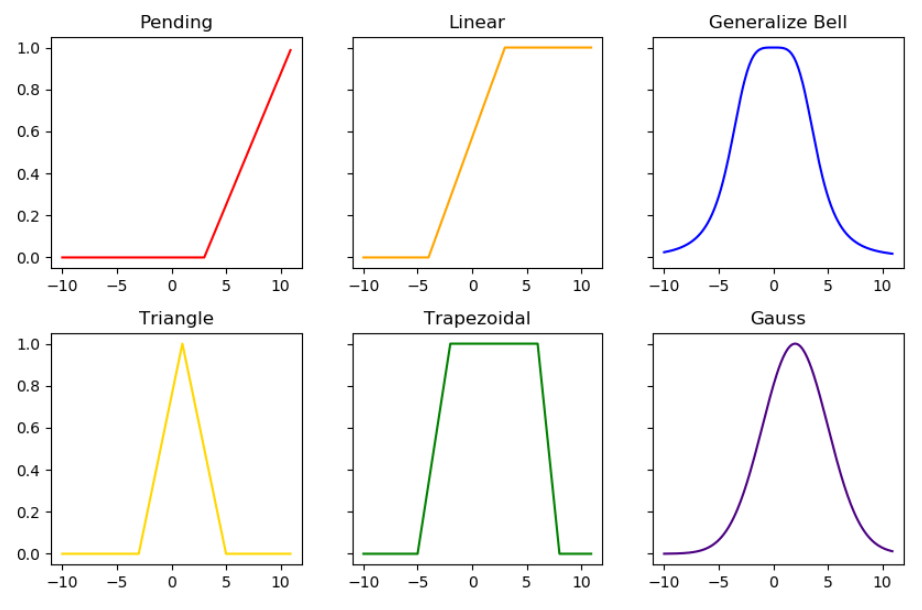
\includegraphics[scale = 0.7]{images/membership_functions.png}
    \caption{Alcuni tipi diffusi di funzioni di appartenenza - da \cite{30}.}
    \label{membership_functions}
\end{figure}

\subsection{Metodo kernel} \label{kernel}
La funzione kernel è un oggetto matematico ampiamente utilizzato in congiunzione con le support vector machine \cite{28} per problemi di natura non lineare, tuttavia è applicabile anche a numerosi altri contesti, ad esempio la kernel Principal Component Analysis \cite{29}.
\\
Questa metodologia prende il nome di \textit{kernel trick} e consiste nel mappare i punti dallo spazio originale a uno spazio a dimensionalità superiore o infinita, dove il problema diventa lineare.
Tale tecnica si appoggia a una funzione kernel, una funzione simmetrica 
\begin{center}
    $k: \mathcal{X} \times \mathcal{X} \rightarrow \mathbb{R}$
\end{center} 
tale che esiste uno spazio lineare $\mathcal{H}$, detto \textit{spazio delle feature}, in cui è definito un prodotto scalare $<$ ·, · $>$ e una funzione $\mathit{\Phi }: \mathcal{X} \rightarrow \mathcal{H}$ per cui:
\begin{center}
    $k(x,y) = <\mathit{\Phi}(x), \mathit{\Phi}(y)>$ dove $x \in \mathcal{X}$ e $y \in \{-1,1\}$.
\end{center}
I dati vengono, quindi, rappresentati tramite dei confronti di coppie, misurando l'equivalente di una misura di similarità: all'aumentare di $k(x,y)$, $x$ e $y$ sono da considerarsi maggiormente  ``simili''.
\\
Inoltre, tramite l'utilizzo di questo metodo, la dimensionalità dei dati dipende solo dal numero di oggetti e non dalla loro dimensione vettoriale.
\\
Esistono diversi tipi di kernel, ad esempio lineare, polinomiale, iperbolico, gaussiano e molti altri ancora.

\subsection{Tipi di kernel}
In letteratura è presente un'importante varietà di kernel ed essi si distinguono per il tipo di funzione $k(x,y)$ utilizzata. Seguono, dunque, alcuni esempi dei kernel più diffusi:

\paragraph{Kernel lineare}
Il kernel lineare usa la funzione
\begin{center}
    $k(x,y) = x \cdot y = \sum\limits_{i=1}^n x_iy_i$
\end{center}
dove $n$ è la dimensione comune di $x$ e $y$.

\paragraph{Kernel polinomiale}
Il kernel polinomiale usa la funzione
\begin{center}
    $k(x,y) = (x \cdot y + 1)^d$
\end{center}
dove $d$ è il grado polinomiale del kernel.

\paragraph{Kernel polinomiale omogeneo}
Il kernel polinomiale omogeneo usa la funzione
\begin{center}
    $k(x,y) = (x \cdot y)^d$
\end{center}
dove $d$ è il grado polinomiale del kernel.

\paragraph{Kernel gaussiano}
Il kernel gaussiano usa la funzione
\begin{center}
    $k(x,y) = e^{-\frac{||x-y||^2}{2\sigma^2}}$
\end{center}
dove $\sigma$ è la deviazione standard.

\paragraph{Kernel iperbolico}
Il kernel iperbolico usa la funzione
\begin{center}
    $k(x,y) = tanh(\alpha x \cdot y + \beta))$
\end{center}
dove $\alpha$ e $\beta$ sono rispettivamente i parametri di scala e offset.

\chapter{Soluzione proposta}
\label{Capitolo 2}
\onehalfspacing
Questo capitolo presenta la soluzione che viene proposta in questa tesi.
Tale soluzione consiste in un sistema di apprendimento supervisionato a partire dall'algoritmo $\bm{\mu}$\textbf{-learn} \cite{1}, il cui funzionamento viene descritto nel Paragrafo \ref{mulearn}.
\\
Segue nel Paragrafo \ref{evaluation} l'illustrazione dei criteri di valutazione dei modelli e nel Paragrafo \ref{generalization} la maniera con cui viene misurata la loro bontà di generalizzazione.
\\
Nel Paragrafo \ref{sistema}, invece, si mostra l'utilizzo che è stato fatto dell'algoritmo sopracitato all'interno del sistema, delineando le fasi che si susseguono nel corso degli esperimenti. Infine nel Paragrafo \ref{predictors} vengono mostrati i due tipi di predittore che sono stati proposti per tali esperimenti.

\section[\texorpdfstring{L'algoritmo $\mu$-learn}%
                        {mu-learn}]% % choose text-only material here
        {L'algoritmo $\bm{\mu}$-learn}  % note use of \bm ("bold math")
\label{mulearn}
$\mu$-\textit{learn} è un algoritmo di Machine Learning che utilizza una procedura originariamente nata nel contesto del support vector clustering \cite{23}.
Essa si colloca nel gruppo di tecniche che lavora su insiemi fuzzy, trattando un problema di ottimizzazione non lineare.
\\
La diversità delle funzioni di appartenenza presenti in letteratura permette una vasta sperimentazione e i parametri associati a tali funzioni possono essere regolati in modo da ottenere forme differenti per gli insiemi fuzzy formati.
Il nome di questo algoritmo suggerisce il suo obiettivo: apprendere $\mu$, la funzione di appartenenza a un determinato insieme fuzzy e generare l'associato modello predittivo.

\subsection{Fuzzificatore} \label{fuzzificatore}
In letteratura i termini \textit{fuzzificazione} e \textit{defuzzificazione} indicano rispettivamente il passaggio da una quantità crisp a una quantità fuzzy e viceversa.
Tale passaggio può avvenire in differenti modi che dipendono dal tipo di fuzzificatore che si utilizza. In questo senso è presente un'ampia scelta di soluzioni: tra quelle più diffuse si menzionano fuzzificatori di tipo lineare ed esponenziale. Nel caso di questi due fuzzificatori, si starebbe stabilendo se il processo di apprendimento sia realizzato facendo decrescere linearmente o esponenzialmente i valori della funzione di appartenenza dal valore 1 fino a 0. Geometricamente, questo equivale a definire una certa misura di distanza nello spazio in cui i punti vengono clusterizzati; con grado di appartenenza maggiore essi saranno raggrupati più densamente nel cluster, dualmente con grado minore, i suddetti punti saranno più distanti dall'insieme.

\subsection{Support vector clustering modificato}
L'assunzione iniziale è quella di disporre di un dataset di punti associati a dei valori binari o ai gradi di appartenenza a un insieme fuzzy sconosciuto.
L'obiettivo è proprio individuare tale insieme e determinare la funzione di appartenenza $\mu$ per approssimarne il grado.
\\
L'algoritmo descritto nel Paragrafo \ref{mulearn} parte dalla tecnica di support vector clustering presente in letteratura \cite{23} e la estende per l'individuazione di insiemi fuzzy. Si tratta di un algoritmo di clustering non parametrico che affronta il problema dell'identificazione del minimo raggio dell'ipersfera di raggio $R$ e centro $a$ che include le immagini di tutti i punti; in particolare, i punti che si trovano sulla superficie di tale ipersfera sono chiamati \textit{support vector} e, nello spazio delle feature, essi dividono i dati in cluster.
\\
L'obiettivo di $\mu$-learn, oltre a trovare la più piccola sfera, è determinare il grado di appartenenza sulla base della distanza tra le immagini dei punti e $a$.
\\
Il problema di ottimizzazione non lineare a cui si accennava nel Paragrafo \ref{mulearn} riguarda, quindi, la minimizzazione del raggio di questa ipersfera.
\\
Quelli che seguono sono i tre vincoli del problema e si distinguono dalla tecnica originale proprio per l'introduzione di $\mu_i$:
\\
\begin{equation}\label{vincolo}
    \mu_i || \mathit{\Phi}(x_i) - a ||^2 \leq \mu_iR^2 + \xi_i \;,
\end{equation}
\begin{equation}\label{vincolo_2}
    (1 - \mu_i) || \mathit{\Phi}(x_i) - a ||^2 \geq (1 - \mu_i)R^2 - \tau_i \;,
\end{equation}
\begin{equation}\label{vincolo_3}
    \xi_i \geq 0, \tau_i \geq 0 \;.
\end{equation}
Il vincolo \ref{vincolo} esprime la condizione necessaria affinchè le immagini dei punti attraverso $\mathit{\Phi}$ appartengano alla sfera mentre il vincolo \ref{vincolo_2} descrive il caso di esclusione dei punti. Infine, il vincolo \ref{vincolo_3} impone dei valori non negativi per le variabili slack che rilassano il problema.
\\
La soluzione originale viene, quindi, estesa minimizzando $R^2 + C\sum(\xi_i + \tau_i)$ tramite (\ref{vincolo}-\ref{vincolo_3}), dove $C$ è un iperparametro, e viene ricavata tramite un solver.
La fase successiva è di indurre il valore della funzione di appartenenza a tale insieme.

\subsection{Induzione di insiemi fuzzy}
Se $F$ è l'insieme fuzzy analizzato, l'algoritmo descritto nel Paragrafo \ref{mulearn} individua un insieme $K \subseteq F$, detto \textit{core}, in cui assegna l'unità come grado di appartenenza dei punti che ne fanno parte. Sulla base del fuzzificatore impostato, poi, l'algoritmo fa decrescere il valore man mano che i punti si allontanano dal core. 
Al fine di visualizzare il comportamento descritto, si mostra in Figura \ref{mulearnplot} un esempio di esecuzione dell'algoritmo e la conseguente rappresentazione del risultato ottenuto:
si assuma che le fake news siano appartenenti a un determinato insieme fuzzy $F$ e si supponga di volerlo individuare tramite la procedura vista in precedenza.
Con un campione di 400 notizie opportunamente preprocessato, è stato eseguito $\mu$-learn con un kernel gaussiano e un fuzzificatore di tipo lineare; successivamente, i risultati sono stati rappresentati in uno spazio bidimensionale applicando ad essi la tecnica di PCA \cite{30}.
\\
Considerando che i punti rossi fanno riferimento alle osservazioni etichettate come fake news e quelli blu alle notizie vere, si osserva la formazione di diverse \textit{curve di livello} che compongono $F$ in prossimità della zona in cui i punti rossi sono maggiormente concentrati.
\\
Al centro, il cerchio più piccolo denota il core $K$ dove i gradi di appartenenza sono uguali a 1, mentre nelle zone periferiche il grado viene diminuito linearmente rispettando i valori delle curve di livello. Tali curve sono utili per distinguere delle fasce che definiscono in maniera ancora più granulare i gradi di appartenenza.
\begin{figure}
    \centering
    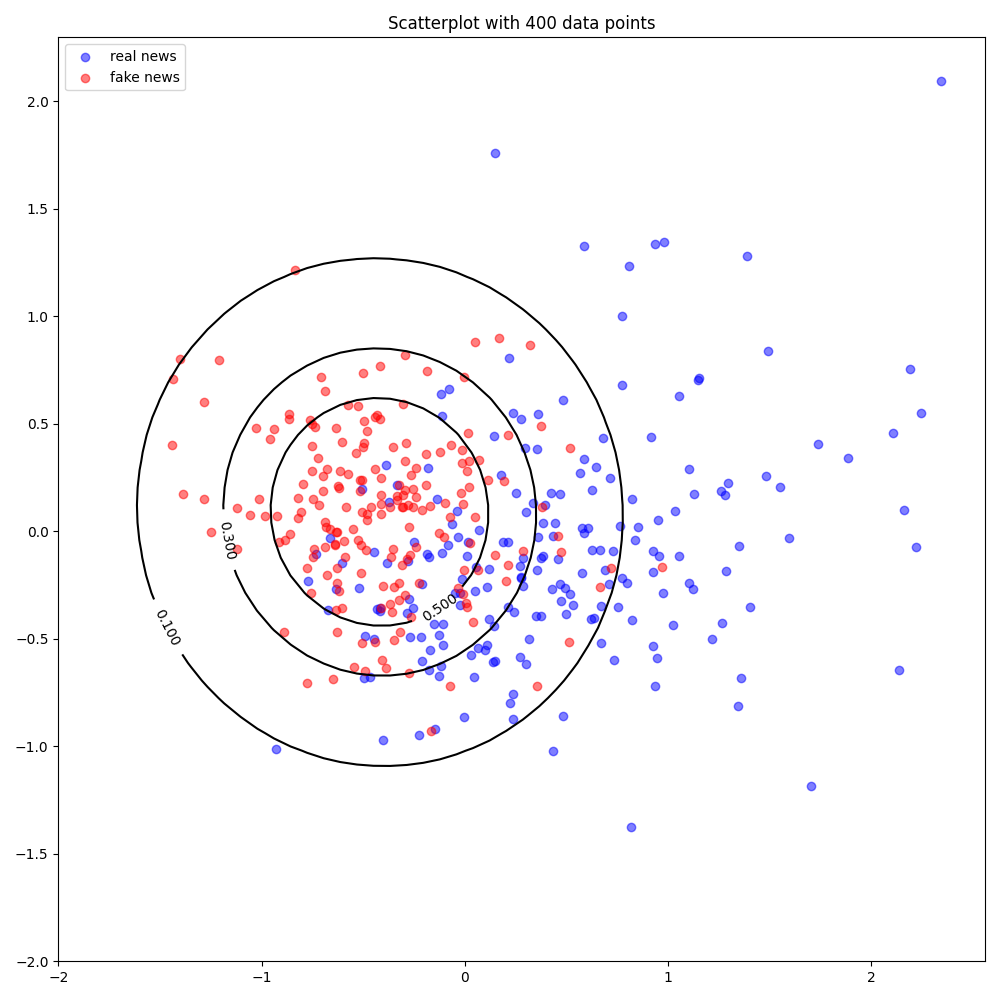
\includegraphics[scale=0.44]{images/mulearn.png}
    \caption{Visualizzazione in uno spazio bidimensionale dei punti (400 osservazioni) e del fuzzy set associato alle fake news indotto da $\mu$-learn. In rosso le notizie echitettate come ``fake'' e in blu come ``vere''.
    \\
    Le curve di livello discriminano le soglie dei gradi di appartenenza dei punti a partire dall'insieme core al centro fino al resto delle osservazioni nelle zone periferiche.}
    \label{mulearnplot}
\end{figure}
\leavevmode\\
La fase di induzione della funzione di appartenenza è lo step in cui l'algoritmo viene effettivamente addestrato tramite i dati etichettati.
\\
L'esito dell'induzione della funzione di appartenenza è influenzato dalla scelta degli iperparametri.

\subsection{Iperparametri}\label{iperparameters}
Gli \textit{iperparametri} sono parametri speciali che non vengono appresi direttamente dall'algoritmo di Machine Learning, al contrario, il loro valore viene assegnato prima dell'addestramento.
Nel contesto considerato da questa tesi si distinguono i seguenti iperparametri: 
\begin{enumerate}
    \item il solver utilizzato,
    \item il tipo di kernel,
    \item eventuali parametri che dipendono dal tipo di kernel,
    \item $C$,
    \item il tipo di fuzzificatore,
    \item eventuali parametri legati al tipo di fuzzificatore.
\end{enumerate}
Nella soluzione proposta in questa tesi, tra le svariate possibilità esistenti, è prevista la scelta tra due solver: \textit{tensorflow} e \textit{gurobi}, che usano strategie differenti per il problema di ottimizzazione non lineare. Il secondo e il terzo iperparametro condizionano indirettamente la forma dell'insieme indotto.
\\
Il parametro $C$ impatta sulla dimensione del core dell'insieme:
all'aumentare di $C$, il core si dilata e incrementa il numero di elementi in esso inclusi.
Inoltre, si è dimostrato sperimentalmente che, al raggiungimento dell'unità da parte di $C$, l'insieme fuzzy tende a un insieme regolare che racchiude i punti del campione le cui etichette sono diverse da zero.
\\
Infine, il quinto e il sesto iperparametro sono legati al processo di fuzzificazione precedentemente definito nel Paragrafo \ref{fuzzificatore}.
Una volta individuato un insieme di valori per ogni iperparametro, è possibile ricorrere a una tecnica per la ricerca dei loro valori ottimali, detta \textit{tuning}.

\paragraph{Tuning} Con tuning si intende l'addestramento di uno stimatore con diverse configurazioni dei suoi iperparametri, al fine di valutare i risultati delle predizioni e, sulla base di essi, scegliere opportunamente il set di valori ottimali per la generazione del modello finale.
\\
Nella soluzione proposta in questa tesi, la fase di tuning è stata concretamente implementata tramite la cosiddetta \textit{grid search}: si tratta di una ricerca del modello migliore che considera una tabella di valori che si desidera esplorare e si basa sulla suddivisione del campione dei dati in \textit{training set}, \textit{validation set} e \textit{test set}.
E' importante, inoltre, che tale campione sia rappresentativo\footnote{Per dataset rappresentativo si intende un campione sufficientemente popolato e bilanciato, ovvero che la distribuzione delle etichette sia approssimativamente uniforme.} del dominio che si intende considerare.
\\
L'algoritmo viene configurato con ogni combinazione della grid search, generando per ciascuna un modello che viene addestrato col training set, un insieme di dati etichettati necessari per formare la memoria del modello predittivo. Successivamente, il modello osserva i dati del validation set, cioè nuove osservazioni del campione senza etichetta, e produce delle predizioni a partire da esse. Tali predizioni vengono, dunque, comparate alle etichette originali per misurare la capacità predittiva del modello; questo viene fatto tramite delle apposite metriche e, sulla base di queste, si sceglie il modello effettivamente più efficace.
\\
Il test set, invece, funge da prova finale per valutare la capacità di generalizzazione del modello su dati mai visti, valutando la bontà delle sue predizioni su di essi.
Esistono tanti modi per dividere i dati nei tre insiemi sopra descritti, uno di questi è la cross validation.


\paragraph{Cross validation} 
La \textit{cross validation} è una tecnica che consiste nel partizionare il dataset in $k$ \textit{fold} equiampi, effettuare altrettante iterazioni e, per ciascuna, considerare l'$i$-esima fold come validation set e le restanti $k-1$ come training set per addestrare il modello generato.
\\
In questo caso esistono diverse scuole di pensiero sulla percentuale che si preferisce impostare per la suddivisione in fold.
\\
Indirettamente, definire ogni combinazione delle fold equivale a definire un nuovo modello, pertanto fare una cross validation $k$-fold significa generare $k$ modelli.
\\
Questa tecnica ha il vantaggio di massimizzare l'utilizzo dei dati, utilizzando a turno ogni fold come validation set e, dunque, consentendo di eseguire l'algoritmo su più casi.

\section{Valutazione dei modelli}\label{evaluation}
La scelta dei modelli si basa su uno o più criteri di valutazione e, tipicamente, avviene tramite delle metriche di accuratezza o attraverso delle misure di errore del predittore generato.
\\
Il range di possibilità esistenti in questo senso è molto ampio e la motivazione che porta a preferire una soluzione piuttosto che un'altra dipende strettamente dal tipo di predittore che si intende costruire: un classificatore binario, ad esempio, porta inevitabilmente a ragionare in termini di accuratezza, andando a valutare in che percentuale il modello classifica correttamente le nuove osservazioni.
Partendo dal presupposto che in questo contesto si possono avere due valori possibili, si distingue in classificazione ``positiva'' e ``negativa'', e si costruiscono i due casi di predizione corretta, \textit{veri positivi} e \textit{veri negativi}, e i due casi di errore, \textit{falsi positivi} e \textit{falsi negativi}.
\\
In un contesto differente, come ad esempio quello della regressione, non è più possibile basare la precisione di un modello sui concetti fin sopra descritti, poiché entra in gioco quella che è la quantificazione dell'errore. L'errore è una misura del discostamento che si verifica tra una predizione e la ground truth, ossia l'effettivo valore delle etichette nel dominio di conoscenza considerato.
Ricorrere a una misura di questo tipo, invece, consente di descrivere quanto sia rilevante l'errore compiuto dal predittore e stabilire se sia numericamente accettabile per la scelta finale del modello.

\subsection{Matrice di confusione}
Quando si mira ad ottenere un classificatore, uno strumento molto utilizzato per valutare la sua precisione è la matrice di confusione, una struttura dati che analizza le predizioni e le divide nelle quattro classi menzionate nel paragrafo precedente. 
Il caso più semplice è quello mostrato in Figura \ref{confusion} in cui si considera delle etichette binarie.
\\
Nel contesto di classificazioni multi-classe è sufficiente estendere la matrice ottenendo sulla diagonale il numero di predizioni corrette e nel resto della matrice i vari casi di errore con cui è possibile capire quali classi vengano più o meno facilmente confuse. 

\begin{figure}
    \centering
    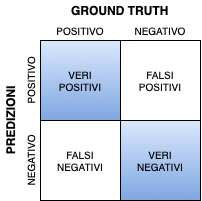
\includegraphics[scale=0.7]{images/confusion matrix.png}
    \caption{Matrice di confusione su classificazione binaria. Nell'ambito considerato in questa tesi la classificazione ``positiva" può riguardare il fatto che una notizia sia fake, dualmente quella ``negativa" si riferirà alle notizie vere.}
    \label{confusion}
\end{figure}

\subsection{Precision, Recall e F1}\label{erroreclass}
Nel contesto della classificazione è possibile calcolare delle misure quantitative per valutare la bontà di un predittore e quelle di \textit{precision}, \textit{recall} e \textit{F1} sono basate sul numero di veri positivi, veri negativi, falsi positivi e falsi negativi.

\paragraph{Precision}
Il valore di \textit{precision} misura la frazione di predizioni positive indovinate dal classificatore. Nell'esempio delle fake news si potrebbe interpretare questa misura come la percentuale di notizie classificate come fake che effettivamente sono false.
\begin{equation}
\frac{Veri\,Positivi}{Veri\,Positivi + Falsi\,Positivi}
\end{equation}

\paragraph{Recall}
La \textit{recall} quantifica il numero di predizioni positive corrette rispetto a tutte le osservazioni positive. Ricollegandosi alle fake news, la recall rappresenterebbe la percentuale di tutte le notizie fake del dataset che sono state individuate dal classificatore.
\begin{equation}
\frac{Veri\,Positivi}{Veri\,Positivi + Falsi\,Negativi}
\end{equation}

\paragraph{F1}
Dal momento che le precedenti quantità rappresentano due facce della stessa medaglia, il punteggio \textit{F1} nasce con l'intento di combinarle tramite la media armonica.
\begin{equation}
\frac{2 \times (Precision \times Recall)}{Precision + Recall}
\end{equation}

\subsection{MSE e RMSE}\label{erroreregr}
Il concetto di accuratezza di un modello non è sempre applicabile, specialmente se si considera un tipo di predittore che produce valori continui\footnote{Qui il termine ``continui'' è da intendersi da un punto di vista puramente teorico, in quanto a livello informatico si tratta comunque di un intervallo di valori discreto, derivante dalla limitata capcità di memoria di un calcolatore.}. In questi casi si ricorre a delle misure del concetto di \textit{errore}, ossia la quantità che descrive quanto il valore della predizione sia deviato rispetto alla ground truth.
In questa tesi sono state utilizzate le metriche di \textit{mean squared error} e di \textit{root mean squared error}.
\\
Si fissi il dataset $S$ formato da tutte le coppie $(\mathbf{x_i},y_i) \; \forall\,i=1, ..., m$, dove $\mathbf{x_i}$ indica il vettore delle feature, $y_i$ l'etichetta, $i$ l'indice di scorrimento delle osservazioni e $m$ è la dimensione del dataset:
\paragraph{MSE} L'errore quadratico medio è definito come
\begin{equation}
    \frac{1}{m}\sum\limits_{j=1}^m (\hat{y_j} - y_j)^2
\end{equation}
dove $\hat{y_j}$ è la predizione.
\paragraph{RMSE}
Al fine di portare il valore dell'errore ad avere lo stesso ordine di grandezza delle predizioni può essere utile sfruttare l'RMSE, definito come 
\begin{equation}
    \sqrt{MSE}
\end{equation}
\\

\section{Bontà di generalizzazione di un modello}\label{generalization}
Nell'ambito del Machine Learning, generare un modello predittivo affidabile non significa selezionare semplicemente il modello che ottiene i risultati migliori bensì quello che si adatta meglio ai dati.
Questa capacità di adattamento consente di valutare quella che viene definita la \textit{bontà di generalizzazione} che il modello ha sui dati che non ha mai visto. Da questo punto di vista, un modello con una buona capacità di generalizzazione è in grado di intuire correttamente le etichette dei dati perchè è riuscito ad estrarre efficacemente la relazione di dipendenza tra le feature e le etichette target desiderate.
A volte, questo meccanismo viene raggiunto sui dati di addestramento tramite una continua regolazione degli iperparametri nella fase di tuning, tuttavia questo rischia di causare la generazione di un modello che su quel tipo di dato riesce a ottenere buoni risultati ma che ha una bassa capacità di generalizzazione su altri poiché, più che formare la sua esperienza su concrete relazioni dei dati, ha raggiunto l'obiettivo tramite un eccessivo incremento della complessità.
\\
Gli iperparametri determinano, infatti, i gradi di libertà del modello ottenuto e la loro numerosità ha un impatto sulla complessità del modello: avere molti iperparametri rischia di complicarlo eccessivamente, dualmente, averne pochi, lo rende potenzialmente troppo semplice. 
Sulla base di queste premesse si introducono, quindi, i concetti di \textit{overfitting} e \textit{underfitting}.

\subsection{Overfitting e underfitting}
Si distinguono modelli che soffrono di \textit{underfitting} quando hanno errore alto sul training set e sul test set, tipicamente questo è causato da un'eccessiva semplificazione del modello o da una quantità di dati di addestramento insufficiente.
\\
Al contrario, modelli che soffrono di \textit{overfitting} sono troppo complessi e mostrano un errore basso sul training set ma alto sul test set, evidenziando una scarsa capacità di generalizzazione.
\\
In letteratura, il problema è descrivibile anche in termini di equilibrio tra \textit{bias} e \textit{variance error} \cite{31}: l'underfitting è il risultato del prevalere del bias error sul variance error; l'overfitting, invece, è causato dal dominare del variance error sul bias error.
Di conseguenza, al fine di trovare un compromesso per controllare questo tipo di problematica, è necessario avere una giusta complessità del modello, associata a un campione di dati sufficientemente grande.
\\
In Figura \ref{underfittingoverfitting} viene riportata una visualizzazione dei due fenomeni in uno spazio lineare. Nell'esempio viene mostrato un regressore lineare che cerca di apprendere la relazione tra i punti, nel primo caso un'eccessiva semplificazione del modello causa un ampio errore mentre nel secondo si ha un sovradattamento del modello che lo rende poco robusto a nuove osservazioni.
Un altro aspetto che non dipende dalla complessità del modello e a cui, però, occorre prestare comunque attenzione è il fenomeno di \textit{data leakage}.

\begin{figure}
\centering
    \begin{minipage}{0.48\textwidth}
        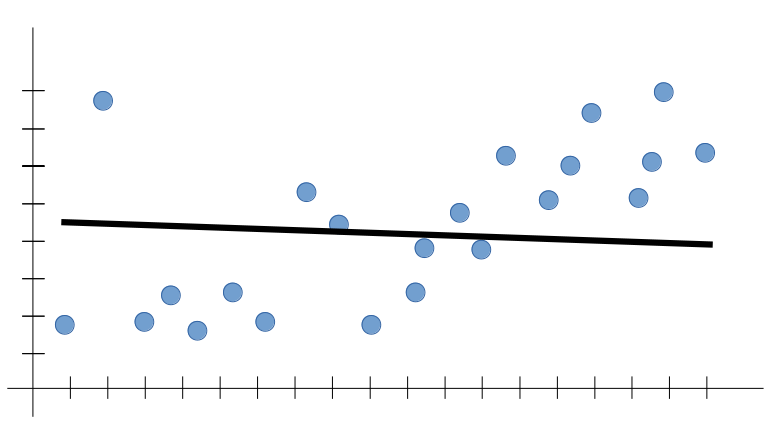
\includegraphics[width=\linewidth]{images/underfitting.png}
    \end{minipage}
    \begin{minipage}{0.48\textwidth}
        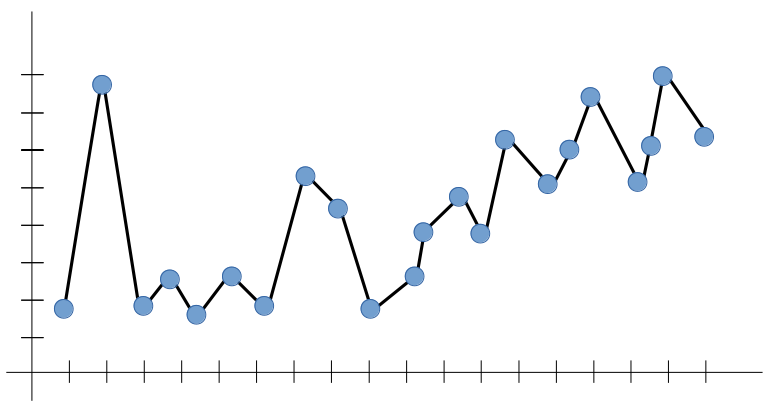
\includegraphics[width=\linewidth]{images/overfitting.png}
    \end{minipage}
    \caption{Esempio di regressore lineare che nel primo caso evidenzia problemi di underfitting mentre nel secondo di overfitting - Fonte: https://towardsdatascience.com/what-are-overfitting-and-underfitting-in-machine-learning-a96b30864690.}
    \label{underfittingoverfitting}
\end{figure} 

\paragraph{Data leakage} Per \textit{data leakage} si intende lo scenario in cui il training set viene contaminato dal test set. In altre parole violare la proprietà di disgiunzione tra questi due tipi di insiemi causa un eccessivo adattamento del modello sui dati di allenamento e, di conseguenza, performa molto bene su questi ultimi ma molto male su osservazioni nuove.
Questa è la ragione per cui il partizionamento del campione in training, validation e test set deve essere fatto rendendo tali insiemi esclusivi fra loro.

\section{Il sistema}
\label{sistema}
In questo paragrafo si mostra ad alto livello l'architettura della soluzione proposta in questa tesi, presentando prima i nodi che la compongono e poi descrivendo come sia stato utilizzato l'algoritmo $\mu$-learn nel contesto del riconoscimento delle fake news.
Nella seconda parte viene, invece, spiegato come i nodi in questione comunichino fra loro e quali file vengano generati durante l'utilizzo del sistema. Sarà, quindi, obiettivo del Capitolo \ref{Capitolo 3} illustrare più a basso livello l'implementazione del sistema e descrivere nel dettaglio i nodi che vi appartengono.
\\
Per gestire la pluralità dei casi nella forma dell'input, il sistema definisce un formato standard per i dataset che andrà a trattare: il dataset ideale è un dataframe che contiene in forma tabulare osservazioni relative a dati testuali che, nell'ambito trattato da questa tesi, possono essere il corpo delle notizie o i titoli.
Tali osservazioni sono etichettate con valore 1 se si tratta di una notizia fake, 0 altrimenti.
\\
L'obiettivo di $\mu$-learn sarà, quindi, indurre l'insieme fuzzy delle fake news inizialmente sconosciuto ed apprendere la funzione di appartenenza ad esso associata.
\subsection{Architettura}\label{architecture}
L'architettura del sistema è composta da tre nodi: 
\begin{enumerate}
    \item il preprocessing del dataset,
    \item la selezione dei modelli migliori,
    \item la visualizzazione dei dati.
\end{enumerate}
Segue, quindi, una breve descrizione di ciascun nodo più nel dettaglio.

\paragraph{Dataset preprocessing} All'inizio di questa fase ci sono tre possibili scenari: i) il dataset rispetta il formato, ii) il dataset è formattato diversamente e dunque necessita di una fase di rielaborazione per poter essere utilizzabile, iii) il dataset viene generato dal sistema stesso.
In altre parole, nel secondo caso è necessario rendere la forma dell'input compatibile col formato predefinito; questo viene fatto da un modulo che ha la funzione di estrarre le informazioni fondamentali e di formare con esse il dataframe desiderato.
A questo punto interviene la vera e propria fase di preprocessing che consiste nell'eseguire una pipeline di operazioni che hanno l'obiettivo di preparare il dataset alla fase successiva.
\\
Le operazioni in questione includono le tecniche di elaborazione del linguaggio naturale descritte nel Capitolo \ref{Capitolo 1} e la cui implementazione viene illustrata nel dettaglio nel Capitolo \ref{Capitolo 3}.
\\
La pipeline che assembla tali operazioni e che le esegue in sequenza viene opportunamente configurata a seconda delle esigenze per attivare o disattivare gli step per l'elaborazione dei dati, anche in base allo scenario considerato.
\\
Al termine del preprocessing, un nuovo dataset viene creato e scritto su file, per il suo utilizzo in un secondo momento. L'intero processo viene schematizzato in Figura \ref{preprocessmodule}.

\begin{figure}
    \centering
    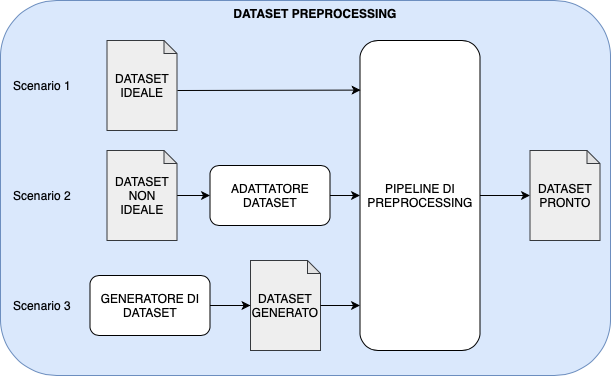
\includegraphics[scale=0.6]{images/preprocessingmodule.png}
    \caption{Primo nodo dell'architettura, il preprocessing dei dati, secondo i tre possibili scenari.}
    \label{preprocessmodule}
\end{figure}

\paragraph{Model selection}
La fase di model selection si occupa di individuare il modello ideale tenendo presente le considerazioni relative alla valutazione della capcità predittiva e alla bontà di generalizzazione dei modelli fatte nei Paragrafi \ref{evaluation} e \ref{generalization}.
\\
Al fine di rendere computazionalmente più agevole l'esecuzione degli esperimenti si è optato per isolare ciascun nodo per permettere, ad ogni step, la scrittura in memoria persistente dell'output. Nel caso della model selection risulta particolarmente conveniente disporre di un dataset precedentemente preprocessato su cui impostare la selezione dei modelli in quanto, innanzitutto potrebbe richiedere notevole tempo per terminare, e soprattutto lo stesso campione preprocessato potrebbe essere utilizzato più volte.
\\
I modelli ottimali vengono generati tramite la tecnica della cross validation annidata\footnote{La cross validation annidata è un'estensione della versione riportata nel Paragrafo \ref{iperparameters} che effettua un'ulteriore cross validation interna per combinare la rotazione delle fold a una ricerca degli iperparametri ottimali, nel caso di questa tesi ciò è avvenuto tramite la grid search.} e, per ciascuna iterazione, viene fatta una \textit{grid search} per indagare quali siano i migliori modelli sulla base del test error ottenuto.
\\
Alla fine di questa operazione vengono ricavati, infatti, i modelli che si sono adattati meglio ai dati e fornita la relativa configurazione degli iperparametri.
\\
\'E in questa fase che si colloca l'utilizzo di $\mu$-learn in quanto le configurazioni della grid search riguardano gli iperparametri di tale algoritmo.
I modelli selezionati vengono, dunque, serializzati per permettere il loro riutilizzo in un secondo momento; più precisamente, questo avviene nel terzo nodo di visualizzazione dei dati in cui si vuole valutare il loro comportamento.
\\
In Figura \ref{selectionmodel} viene mostrata la rappresentazione del funzionamento sopra descritto.
\begin{figure}
    \centering
    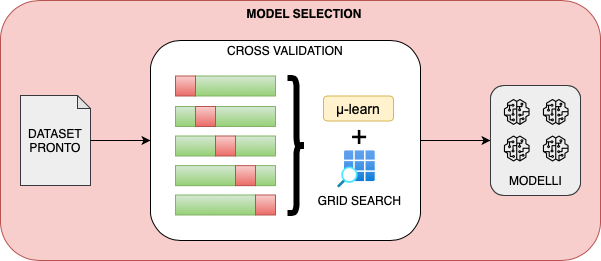
\includegraphics[scale=0.6]{images/modelselectionmodule.png}
    \caption{Secondo nodo dell'architettura, la selezione dei modelli.}
    \label{selectionmodel}
\end{figure}

\paragraph{Data visualization} 
Nella parte di visualizzazione dei dati, i modelli vengono deserializzati per poterli riutilizzare al fine di operare un'analisi descrittiva.
Tale analisi coinvolge principalmente i gradi di appartenenza approssimati dai modelli generati dal sistema, valutando la bontà delle predizioni da essi effettuate.
\\
Il criterio con cui viene valutata la correttezza delle predizioni consiste nell'utilizzare le misure quantitative descritte nei Paragrafi \ref{erroreclass} e \ref{erroreregr}. Si sottolinea, inoltre, che in questa fase vengono effettuati dei confronti con una determinata \textit{baseline}, ovvero uno o più stimatori di riferimento le cui predizioni vengono valutate sugli stessi dati trattati da $\mu$-learn, per poter fornire un ulteriore metro di paragone. Come mostrato in Figura \ref{datavisualization}, l'analisi può interagire nuovamente col dataset di partenza per poter visionare quelle osservazioni che causano incertezza nelle predizioni. Complessivamente, il terzo nodo è importante per poter estrarre maggior conoscenza dall'ambito preso in considerazione. Tutte le conclusioni tratte dall'analisi descrittiva, infatti, vengono riassunte in un report e sulla base di esso, si può eventualmente decidere se ricominciare gli esperimenti.

\begin{figure}
    \centering
    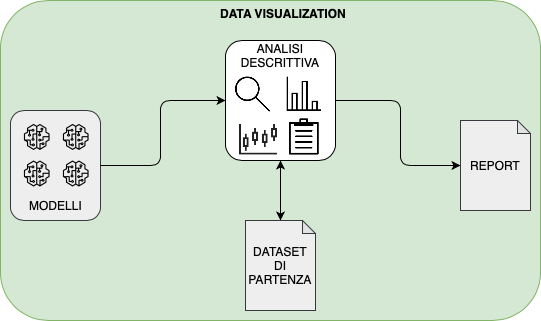
\includegraphics[scale=0.6]{images/datavisualizationmodule.png}
    \caption{Terzo nodo dell'architettura, la visualizzazione dei dati.}
    \label{datavisualization}
\end{figure}

\subsection{Funzionamento del sistema}
In questo paragrafo si descrive come funziona il sistema nella sua complessità e come esso sia stato utilizzato per produrre dei risultati.
\begin{figure}[!ht]
    \centering
    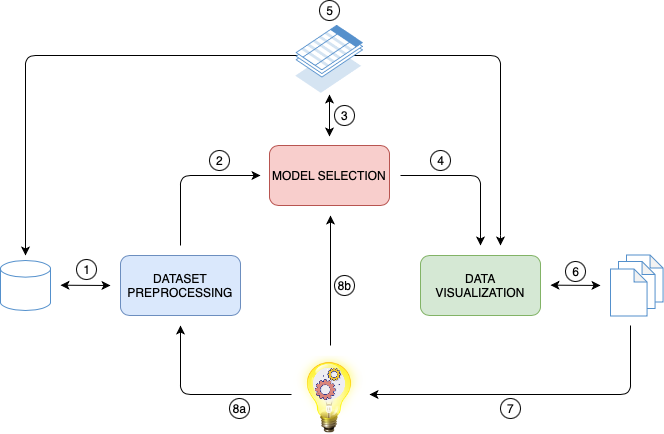
\includegraphics[scale=0.6]{images/cycle.png}
    \caption{Schema del flusso di comunicazione all'interno del sistema.}
    \label{cycle}
\end{figure}
\\
In Figura \ref{cycle} viene raffigurato il flusso di comunicazione all'interno del sistema, numerato passo per passo: 
\begin{enumerate}
    \item il processo ha inizio quando si dispone di un dataset, ottenuto in uno dei modi visti in precedenza, e viene così acquisito dal primo nodo per il preprocessing;
    \item  il nodo effettua il preprocessing del dataset e ne produce uno nuovo che viene opportunamente scritto su file per permettere la successiva lettura da parte del nodo di model selection;
    \item i modelli predittivi ottimali sono stati trovati, serializzati e il sistema aggiorna la storia degli esperimenti, documentata in un registro dedicato. Lo scopo del registro è catalogare i modelli e i loro dati associati tramite l'informazione di data e ora;
    \item i modelli vengono deserializzati e usati per l'analisi descrittiva delle predizioni;
    \item tramite il registro, il sistema è in grado di risalire al dataset utilizzato per ottenere i relativi modelli e, dunque, completare l'analisi;
    \item il modulo per la visualizzazione dei dati fornisce un report che viene aggiunto a quelli associati agli altri esperimenti;
    \item il report permette di analizzare il comportamento dei modelli e individuare delle possibili configurazioni da testare per i nuovi esperimenti;
    \item se si desira fare nuovi esperimenti
    \\
    a) ripartendo dal preprocessing dei dati, è necessario ricominciare l'esperimento dall'inizio, andando a modificare i parametri in questione;
    \\
    b) modificando il modo in cui viene fatta la grid search, si regolano i relativi valori a partire dalla model selection.
\end{enumerate}

\section{Tipi di predittore considerati}\label{predictors}
Le considerazioni fatte nei Paragrafi \ref{erroreclass} e \ref{erroreregr} portano a domandarsi quale tipo di predittore sia il caso di considerare per il problema delle fake news.
\\
Sono state esplorate due possibilità: la pura induzione della funzione di appartenenza e un classificatore binario derivato da tale induzione.
Siano $\lambda$ e $\omega$ i due predittori appena presentati, si definisce il primo predittore come
\begin{center}
    $\lambda$: $\mathbb{R}^h \rightarrow \mu$
\end{center}
con $\mu \in [0,1]$ e dove $h$ è il numero di feature; sia $x$ una generica osservazione del dataset, il secondo predittore è definito come
\begin{center}
    $\omega(x) = \begin{cases} 1 & \mbox{se } \lambda(x) >= 0.5, \\ 0 & \mbox{altrimenti.} \end{cases}$
\end{center}
Ne consegue che per $\lambda$ risultano più appropriate le misure di MSE e RMSE, mentre per $\omega$ sono state scelte le metriche di precision, recall e F1\footnote{In realtà si tratta di una versione leggermente modificata: si tratta di calcolare le misure di precision, recall e F1 pesando il numero di veri positivi e falsi positivi con $\mu$ e il numero di falsi negativi per $1-\mu$.}.

\chapter{Implementazione}
\label{Capitolo 3}
\onehalfspacing
Il Capitolo \ref{Capitolo 3} tratta l'implementazione della soluzione proposta nel capitolo precedente. Nel Paragrafo \ref{datasethandle} si descrive la prima parte inerente alle modalità con cui si gestiscono i vari scenari relativi al tipo di dataset che si ha a disposizione.
\\
All'interno del Paragrafo \ref{pp} viene illustrata la pipeline di preprocessing, soffermandosi su ognuno degli step che la compongono; il Paragrafo \ref{modelselection}, invece, descrive come è stata implementata la parte di model selection tramite la grid search.
\\
Infine, nel Paragrafo \ref{datavisualizationimpl} viene descritta la fase di visualizzazione dei dati.

\section{Gestione dei dataset}\label{datasethandle}
Il sistema di apprendimento supervisionato proposto in questa tesi ha bisogno di molti esempi per affinare le predizioni, pertanto sono stati previsti più scenari al fine di massimizzare la mole di dati destinata all'addestramento. Principalmente, le vie percorse sono state due: utilizzare un dataset acquisito da terzi oppure generarlo.
Nel primo caso servizi come \textit{Kaggle} hanno facilitato l'individuazione di dataset interessanti, mentre nel secondo è stato implementato un modulo adibito alla generazione artificiale di documenti testuali.

\subsection{Adattatore di dataset}\label{adapter}
Per gestire la diversità della forma dei dati, si è deciso di fissare un formato standard e, in base ad esso, adattare o meno il dataset a disposizione in modo che rispetti tale convenzione. L'obiettivo è facilitare l'esecuzione di tutto il sistema su nuovi dati.
Il sistema descritto nel Paragrafo \ref{sistema} assume, quindi, un dataframe di tre colonne: \textit{index}, \textit{text} e \textit{label}.
\\
L'indice ha la finalità di preservare l'identificatore di ogni osservazione, questo torna particolarmente utile i) quando si vuole analizzare specifiche notizie durante la fase di data visualization; ii) per mantenere il riferimento alla posizione originale delle notizie rimescolate durante lo step di shuffling nel preprocessing.
\\
Il testo riguarda delle possibili sequenze di parole che, nell'ambito delle fake news, possono essere il corpo delle notizie, i titoli o, a seconda del dataset considerato, dei possibili tweet o post sui social media.
\\
L'etichetta ha due forme possibili: un valore binario o un valore compreso nell'intervallo $[0,1]$ per il caso di dataset generati.

\subsection{Generatore di dataset}\label{generator}
Oltre a poter trattare osservazioni con etichette categoriali relative a notizie che sono fake o meno, è possibile considerare anche dei dati etichettati con il grado di appartenenza. Un tipo di dataset così organizzato è più difficile da reperire; di conseguenza, al fine di produrre degli esperimenti più esaustivi, si è deciso di implementare un modulo per la generazione di dataset con il grado di appartenenza. Il modulo in questione si basa sulla tecnica \textit{LDA}, \textit{Latent Dirichlet Allocation} \cite{20} per la creazione di documenti testuali come misture di parole appartenenti a topic diversi. 
Si consideri, quindi, $t_1$ il topic delle notizie vere e $t_2$ quello delle notizie fake; ciascun topic è rappresentato da un insieme di parole $P_i$ che lo caratterizza. Per semplicità, è stato considerato prima il caso di $P_1 \cap P_2 = \emptyset$ e poi quello dell'intersezione non vuota.
\\
La tecnica prevede la generazione di $m$ documenti composti da $n$ parole estratte dai topic; si definisce, quindi, grado di appartenenza ``atteso'' la probabilità $\mu_i$ di successo di una distribuzione binomiale che una parola $p_j \in P_1$ oppure $p_j \in P_2$, con $i=1, ..., m$ e $j=1, ..., n$, e $B, Z$ due variabili casuali che seguono rispettivamente la distribuzione binomiale e la distribuzione di Zipf \cite{34}. Infine, sia $d$ un'arbitraria distribuzione di probabilità, il funzionamento dello strumento di supporto fin sopra descritto viene mostrato nell'Algoritmo \ref{lda}.
\begin{algorithm}
\caption{procedura del \texttt{generatore di dataset}}
\label{lda}
\hspace*{\algorithmicindent} \textbf{Procedure} generator($m$, $n$, $d$, $P$)
\newline
\hspace*{\algorithmicindent} \textbf{Input}: $m$ è il numero di documenti, $n$ il numero di parole per ogni documento, $d$ è la distribuzione arbitraria, $P$ è la lista che contiene $P_1$ e $P_2$: gli insiemi di parole che rappresentano i due topic
\newline
\hspace*{\algorithmicindent} \textbf{Output}: $m$ documenti testuali artificiali
\begin{algorithmic}[1]
\STATE documents = [ ]
\FOR{$i$ in $1, ..., m$}
\STATE $\mu_i$ = extraction($d$)
\STATE document = [ ]
\STATE document.membership = $\mu_i$
\FOR{$j$ in $1, ..., n$}
\STATE $B$ = extraction(binomial, probability = $\mu_i$)
\STATE $Z$ = extraction(zipf)
\STATE word = $P$[$B$][$Z$]
\STATE document.add(word)
\ENDFOR
\STATE documents.add(document)
\ENDFOR
\RETURN documents
\end{algorithmic}
\end{algorithm}
In pratica, si tratta di un processo non deterministico di estrazione delle parole, in cui la variabile $Z$ indica la parola estratta, una volta fissato il topic scelto tramite $B$.
\\
L'obiettivo del generatore è testare la capacità predittiva di $\mu$-learn e capire la potenzialità di questo approccio nell'avvicinarsi al grado di appartenenza atteso.

\section{Pipeline di preprocessing}\label{pp}
Per la fase di preprocessing è stata predisposta una pipeline, ovvero un insieme di operazioni eseguite consecutivamente.
\\
La sequenza di operazioni viene configurata al momento dell'esecuzione tramite un'opportuna parametrizzazione degli step della pipeline.
\\
Ogni operazione segue il pattern di implementazione della libreria \textit{scikit-learn} che prevede di separare le procedure di \textit{fit} e \textit{transform}: esse definiscono rispettivamente la parte di apprendimento dei dati, quando richiesta, e quella di effettiva trasformazione dell'input in un output processato.
Adottare questa convenzione rappresenta un vantaggio per poter accedere alle funzioni della suddetta libreria parametrizzando le operazioni.
Inoltre, il codice organizzato in questa maniera si presta bene a future estensioni e favorisce la sua manutenibilità poiché rispetta il criterio della \textit{Separation of Concerns}, concetto cardine nell'ambito dell'Ingegneria del software \cite{32}.
\\
Quella che segue è la lista dei parametri della pipeline che al momento della configurazione è possibile attivare a seconda delle esigenze:
\begin{itemize}
    \item Lowercase,
    \item Rimozione dei duplicati,
    \item Lemmatizzazione,
    \item Tokenizzazione,
    \item Rimozione del rumore,
    \item Stemming,
    \item Rimozione delle stop word,
    \item Word2Vec,
    \item Aggregazione,
    \item Doc2Vec.
\end{itemize}
Addizionalmente si considera anche uno step finale di Shuffling che fa una permutazione delle righe.
\\
In generale, le operazioni non sono tutte compatibili, al contrario, alcune sono tra di loro esclusive, come Word2Vec e Doc2Vec, oppure la lemmatizzazione e lo stemming.
Inoltre, l'ordine con cui esse vengono applicate è determinante per la rielaborazione del testo: è più semplice rimuovere il rumore analizzando i token piuttosto che le stringhe di intere frasi, ecco perchè la tokenizzazione avviene tipicamente nei primi step della pipeline. Un altro esempio è quello dell'aggregazione che, come visto nei Paragrafi \ref{w2v} e \ref{d2v}, è necessaria solo in caso di utilizzo di Word2Vec.
\begin{figure}
    \centering
    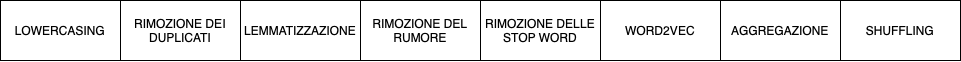
\includegraphics[scale=0.45]{images/pipeline.png}
    \caption{Esempio di configurazione di una pipeline di preprocessing.}
    \label{pipeline}
\end{figure}
In Figura \ref{pipeline} viene mostrato un esempio di pipeline che è stata frequentemente utilizzata durante gli esperimenti. Si noti come in questo tipo di configurazione non sia necessario includere lo step di tokenizzazione in quanto la lemmatizzazione prevede una suddivisione in token che garantisce lo stesso risultato.

\subsection{Lowercasing}
Il \textit{lowercasing} è una tecnica che consiste nel trasformare una stringa di testo in una stringa composta unicamente da caratteri minuscoli.
\\
\\
\textbf{Input}: dataframe di stringhe,
\begin{center}
    \begin{tabular}{|c|c|}
    \hline
    \textbf{index} & \textbf{text} \\
    \hline
         0 & `\textit{This is a sentence. Lowercasing is going to do its job.}'\\
         1 & `\textit{This is another sentence.}'\\
    \hline
    \end{tabular}
\end{center}
\textbf{Output}: dataframe di stringhe,
\begin{center}
    \begin{tabular}{|c|c|}
    \hline
    \textbf{index} & \textbf{text} \\
    \hline
         0 & `\textit{this is a sentence. lowercasing is going to do its job.}'\\
         1 & `\textit{this is another sentence.}'\\
    \hline
    \end{tabular}
\end{center}

\subsection{Rimozione dei duplicati}
In questo caso, per duplicati si intende le osservazioni ripetute nel dataset ed esse vengono rimosse dal dataframe in questo step.
\\
\\
\textbf{Input}: dataframe di stringhe,
\begin{center}
    \begin{tabular}{|c|c|}
    \hline
    \textbf{index} & \textbf{text} \\
    \hline
         0 & `\textit{This is a duplicate sentence.}'\\
         1 & `\textit{This is a duplicate sentence.}'\\
         2 & `\textit{This is another sentence.}'\\
    \hline
    \end{tabular}
\end{center}
\textbf{Output}: dataframe di stringhe,
\begin{center}
    \begin{tabular}{|c|c|}
    \hline
    \textbf{index} & \textbf{text} \\
    \hline
         0 & `\textit{This is a duplicate sentence.}'\\
         1 & `\textit{This is another sentence.}'\\
    \hline
    \end{tabular}
\end{center}

\subsection{Lemmatizzazione}
La \textit{lemmatizzazione} è la tecnica che ricava da una frase i lemmi che la compongono sulla base della morfologia delle parole.
Questo step include implicitamente la divisione in token.
Si osservi, inoltre, che nel caso di pronomi la lemmatizzazione produce una generica stringa \texttt{-PRON-} in quanto morfologicamente non esiste una base.
\\
\\
\textbf{Input}: dataframe di stringhe,
\begin{center}
    \begin{tabular}{|c|c|}
    \hline
    \textbf{index} & \textbf{text} \\
    \hline
         0 & `\textit{this is a sentence that is going to be split.}'\\
         1 & `\textit{here there is another sentence which confirms it.}'\\
    \hline
    \end{tabular}
\end{center}
\textbf{Output}: dataframe di liste di stringhe,
\begin{center}
    \begin{tabular}{|c|c|}
    \hline
    \textbf{index} & \textbf{text} \\
    \hline
         0 & [\textit{`this', `be', `a', `sentence', `that', `be', `go', `to', `be', `split', `.'}]\\
         1 & [\textit{`here', `there', `be', `another', `sentence', `which', `confirm', `-PRON-', `.'}]\\
    \hline
    \end{tabular}
\end{center}

\subsection{Tokenizzazione}
La \textit{tokenizzazione} è, invece, la pura suddivisione delle frasi in token.
\\
\\
\textbf{Input}: dataframe di stringhe,
\begin{center}
    \begin{tabular}{|c|c|}
    \hline
    \textbf{index} & \textbf{text} \\
    \hline
         0 & `\textit{This is a sentence that is going to be split.}'\\
         1 & `\textit{Here there is another sentence which confirms it.}'\\
    \hline
    \end{tabular}
\end{center}
\textbf{Output}: dataframe di liste di stringhe,
\begin{center}
    \begin{tabular}{|c|c|}
    \hline
    \textbf{index} & \textbf{text} \\
    \hline
         0 & [\textit{`This', `is', `a', `sentence', `that', `is', `going', `to', `be', `split', `.'}]\\
         1 & [\textit{`Here', `there', `is', `another', `sentence', `which', `confirms', `it', `.'}]\\
    \hline
    \end{tabular}
\end{center}

\subsection{Rimozione del rumore}
La \textit{rimozione del rumore} è, a sua volta, scomponibile in molteplici passaggi, ciascuno delegato alla rimozione di uno specifico tipo di rumore.
In tal senso, sono stati implementate le rimozioni di URL, emoji, punteggiatura, numeri, parole contenenti numeri, parole duplicate, e osservazioni vuote nel dataset. 
\\
\\
\textbf{Input}: dataframe di liste di stringhe,
\begin{center}
    \begin{tabular}{|c|c|}
    \hline
    \textbf{index} & \textbf{text} \\
    \hline
         0 & [\textit{`This', `is', `www.unimi.it', `\smiley{}'}, `,', `my', `number', `is', `928792', `.']\\
         1 & [\textit{ }] \\
         2 & [\textit{`My', `username', `is', `fire95'}] \\
    \hline
    \end{tabular}
\end{center}
\textbf{Output}: dataframe di liste di stringhe,
\begin{center}
    \begin{tabular}{|c|c|}
    \hline
    \textbf{index} & \textbf{text} \\
    \hline
         0 & [\textit{`This', `is', `my', `number'}]\\
         1 & [\textit{`My', `username', `is'}] \\
    \hline
    \end{tabular}
\end{center}

\subsection{Stemming}
Lo \textit{stemming} ha l'obiettivo di rimuovere suffissi e prefissi per individuare la radice delle parole.
\\
\\
\textbf{Input}: dataframe di liste di stringhe,
\begin{center}
    \begin{tabular}{|c|c|}
    \hline
    \textbf{index} & \textbf{text} \\
    \hline
         0 & [\textit{`this', `is', `a', `sentence', `that', `is', `going', `to', `be', `split', `.'}]\\
         1 & [\textit{`here', `there', `is', `another', `sentence', `which', `confirms', `it', `.'}]\\
    \hline
    \end{tabular}
\end{center}
\textbf{Output}: dataframe di liste di stringhe,
\begin{center}
    \begin{tabular}{|c|c|}
    \hline
    \textbf{index} & \textbf{text} \\
    \hline
         0 & [\textit{`thi', `is', `a', `sentenc', `that', `is', `go', `to', `be', `split', `.'}]\\
         1 & [\textit{`here', `there', `is', `anoth', `sentenc', `which', `confirm', `it', `.'}]\\
    \hline
    \end{tabular}
\end{center}

\subsection{Rimozione delle stop word}
Come accennato nel Capitolo \ref{Capitolo 1}, si può scegliere di rimuovere le \textit{stop word}, parole molto frequenti all'interno di un documento ma che poco aggiungono alla semantica del testo.
\\
\\
\textbf{Input}: dataframe di liste di stringhe,
\begin{center}
    \begin{tabular}{|c|c|}
    \hline
    \textbf{index} & \textbf{text} \\
    \hline
         0 & [\textit{`thi', `is', `a', `sentenc', `that', `is', `go', `to', `be', `split'}]\\
         1 & [\textit{`here', `there', `is', `anoth', `sentenc', `which', `confirm', `it'}]\\
    \hline
    \end{tabular}
\end{center}
\textbf{Output}: dataframe di liste di stringhe,
\begin{center}
    \begin{tabular}{|c|c|}
    \hline
    \textbf{index} & \textbf{text} \\
    \hline
         0 & [\textit{`thi', `sentenc', `split'}]\\
         1 & [\textit{`anoth', `sentenc', `confirm'}]\\
    \hline
    \end{tabular}
\end{center}

\subsection{Word2Vec}
\textit{Word2Vec} è la prima delle due tecniche di embedding citate in questa tesi che converte ogni parola in un vettore di feature numeriche.
L'esempio considera 96 feature
\\
\\
\textbf{Input}: dataframe di liste di stringhe,
\begin{center}
    \begin{tabular}{|c|c|}
    \hline
    \textbf{index} & \textbf{text} \\
    \hline
         0 & [\textit{`thi', `sentenc', `split'}]\\
         1 & [\textit{`anoth', `sentenc', `confirm'}]\\
    \hline
    \end{tabular}
\end{center}
\textbf{Output}: dataframe di liste di liste di valori float,
\begin{center}
    \begin{tabular}{|c|c|}
    \hline
    \textbf{index} & \textbf{text} \\
    \hline
         0 & [[1.12, ..., -3.6], [-1.83, ..., -2.20], [-0.96, ..., -1.04]] (4 liste di 96 elementi) \\
         1 & [[-0.32, ..., -1.96], [-1.83, ..., -2.20], [0.20, ..., -2.60]] (4 liste di 96 elementi) \\
    \hline
    \end{tabular}
\end{center}

\subsection{Aggregazione}
La fase di \textit{aggregazione} è necessaria nel caso si utilizzi Word2Vec, poiché l'obiettivo finale è ottenere nuovamente un dataframe di vettori.
\\
In questo esempio si mostra l'aggregazione tramite la media dei vettori.
\\
\\
\textbf{Input}: dataframe di liste di liste di valori float,
\begin{center}
    \begin{tabular}{|c|c|}
    \hline
    \textbf{index} & \textbf{text} \\
    \hline
         0 & [[1.12, ..., -3.60], [-1.83, ..., -2.20], [-0.96, ..., -1.04]] (4 liste di 96 elementi) \\
         1 & [[-0.32, ..., -1.96], [-1.83, ..., -2.20], [0.20, ..., -2.60]] (4 liste di 96 elementi) \\
    \hline
    \end{tabular}
\end{center}
\textbf{Output}: dataframe di liste di valori float,
\begin{center}
    \begin{tabular}{|c|c|}
    \hline
    \textbf{index} & \textbf{text} \\
    \hline
         0 & [-0.81, -0.63, ..., -2.24] (96 elementi) \\
         1 & [-0.88, -1.22, ..., -2.22] (96 elementi) \\
    \hline
    \end{tabular}
\end{center}

\subsection{Doc2Vec}
\textit{Doc2Vec} è una soluzione alternativa di embedding per convertire direttamente le frasi in vettori; essa non necessita, infatti, di una fase di aggregazione ma richiede come input un dataframe di stringhe.
L'esempio considera un modello di 20 feature 
\\
\\
\textbf{Input}: dataframe di stringhe,
\begin{center}
    \begin{tabular}{|c|c|}
    \hline
    \textbf{index} & \textbf{text} \\
    \hline
         0 & \textit{`thi sentenc split'}\\
         1 & \textit{`anoth sentenc confirm'}\\
    \hline
    \end{tabular}
\end{center}
\textbf{Output}: dataframe di liste di float,
\begin{center}
    \begin{tabular}{|c|c|}
    \hline
         0 & [0.02, 0.03, ..., 0.04] (20 elementi) \\
         1 & [-0.01, -0.03, ..., 0.03] (20 elementi) \\
    \hline
    \end{tabular}
\end{center}

\subsection{Shuffling}
Fare lo \textit{shuffling} dei dati significa effettuare una permutazione delle righe per assicurarsi che il dataset non segua uno specifico ordine; inoltre, quest'operazione fa sì che i modelli ottenuti rimangano generali, lenendo, quindi, il problema di overfitting.
\\
Secondariamente, quest'operazione fornisce un ulteriore modo per ottenere dei dataset rappresentativi, anche se, come verrà spiegato nel Paragrafo \ref{gs}, esistono altre tecniche che hanno lo stesso obiettivo. 
\\
\\
\textbf{Input}: dataframe preprocessato,
\begin{center}
    \begin{tabular}{|c|c|c|}
    \hline
    \textbf{index} & \textbf{text} & \textbf{label} \\
    \hline
         0 & [0.02, 0.03, ..., 0.04] (20 elementi) & 1 \\
         1 & [-0.01, -0.03, ..., 0.03] (20 elementi) & 1 \\
         2 & [0.04, 0.01, ..., 0.91] (20 elementi) & 0 \\
         3 & [-0.07, 0.31, ..., 0.02] (20 elementi) & 0 \\
    \hline
    \end{tabular}
\end{center}
\textbf{Output}: dataframe preprocessato e rimescolato,
\begin{center}
    \begin{tabular}{|c|c|c|}
    \hline
    \textbf{index} & \textbf{text} & \textbf{label} \\
    \hline
        3 & [-0.07, 0.31, ..., 0.02] (20 elementi) & 0 \\
        0 & [0.02, 0.03, ..., 0.04] (20 elementi) & 1 \\
        2 & [0.04, 0.01, ..., 0.91] (20 elementi) & 0 \\
        1 & [-0.01, -0.03, ..., 0.03] (20 elementi) & 1 \\
    \hline
    \end{tabular}
\end{center}

%\subsection{Normalizzazione}
%Spesso, in letteratura, in una pipeline come %questa è presente anche uno step finale per la %normalizzazione dei dati.
%In questo lavoro di tesi è stato scelto di non %usufruire di tale tecnica per la seguente %ragione: in \cite{36} si 

\section{Selezione dei modelli}\label{modelselection}
Nel processo di apprendimento di un task predittivo vengono generati numerosi modelli; per questa ragione diventa cruciale utilizzare un criterio di selezione di tali modelli come la grid search per ricavare i migliori risultati possibili.

\subsection{Grid search}\label{gs}
La grid search è una tecnica di ricerca del modello migliore che, sostanzialmente, automatizza il processo di tuning.
\\
Il termine grid deriva dal fatto che si preimposta una griglia di valori per tutti gli iperparametri di cui si desidera fare il tuning.
\\
Un esempio di griglia viene mostrato in Tabella \ref{grid}: in questo caso è stato fissato il tipo di fuzzificatore, il tipo di kernel e il tipo di solver, mentre è stato previsto un intervallo di dieci ordini di grandezza per $\sigma$, parametro del kernel gaussiano, e per $C$.
\\
\begin{table}[!h]
\centering
 \begin{tabular}{|c|c|c|c|c|} 
 \hline
\textbf{fuzzificatore} & \textbf{kernel} & \textbf{solver} & $\bm{\sigma}$ & $\mathbf{C}$ 
\\ [0.5ex] 
 \thickhline
 lineare & gaussiano & gurobi & logspace(-5, 5, 11) & logspace(-5, 5, 11) \\ 
 \hline
\end{tabular}
\caption{Esempio di griglia di iperparametri.}
\label{grid}
\end{table}
\leavevmode\\
Chiaramente, più ampio è il set di valori da ottimizzare, più computazionalmente costosa diventa l'esecuzione dell'algoritmo, in quanto necessita di reiterare ulteriormente il processo. In questo senso, l'esempio mostra anche l'evenienza in cui alcuni valori vengono fissati per favorire la ricerca di quelli ottimali per altri parametri, alleggerendo, dunque, il carico computazionale.

\paragraph{k-fold cross validation}
Lo stratagemma utilizzato da questa tecnica consiste nel dividere il dataset $S$ in $k$ partizioni $S_1, S_2, ..., S_k$, dette fold, tali che:
\begin{equation}
     S = \bigcup\limits_{i=1}^{k} S_{i},
\end{equation}
\begin{equation}
    S_i \cap S_j = \emptyset \ \ \forall i \neq j.
\end{equation}
Si denota con $S^{(i)} \equiv S \setminus S_i$ la parte per l'addestramento e $S_i$ la parte per la validazione, come illustrato in Figura \ref{cv}.
Per completezza, nell'Algoritmo \ref{kfold} vengono delineati i passi chiave della procedura: si fa un partizionamento in $k$ fold\footnote{Il partizionamento tipicamente tiene conto della rappresentatività delle fold ottenute: in \textit{Scikit-learn} esistono delle funzioni come \textit{StratifiedKFold} che permettono di operare una suddivisione tale le fold abbiano un rapporto bilanciato delle occorrenze dei valori delle etichette.}, organizzandole in insiemi per il training e per il test, come visto sopra, e per ogni iterazione si genera un modello che viene valutato tramite delle metriche.
\begin{figure}
    \centering
    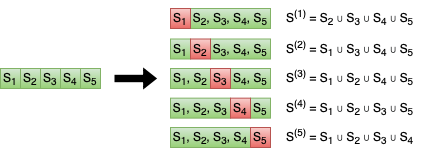
\includegraphics[scale=0.83]{images/cv.png}
    \caption{Schematizzazione del processo di cross validation: in rosso la parte per la validation e in verde la parte per il training.}
    \label{cv}
\end{figure}
\begin{algorithm}
\caption{procedura della \texttt{k-fold cross validation}}
\label{kfold}
\hspace*{\algorithmicindent} \textbf{Procedure} cv($S$, $k$)
\newline
\hspace*{\algorithmicindent} \textbf{Input}: $S$ è il dataset, $k$ il numero di fold
\newline
\hspace*{\algorithmicindent} \textbf{Output}: $k$ modelli
\begin{algorithmic}[1]
\STATE $S_1, S_2, ..., S_k$ = partitioning($S$, $k$)
\FOR{$S_i$ in $S_1, S_2, ..., S_k$}
\STATE test = $S_i$
\STATE train = $S \setminus S_i$
\STATE model = mulearn.fit(train)
\STATE predictions = model.predict(test)
\STATE evaluation = model.evaluate(predictions)
\STATE models.add(model)
\STATE evaluations.add(evaluation)
\ENDFOR
\RETURN models, evaluations
\end{algorithmic}
\end{algorithm}
Per combinare i vantaggi della cross validation con quelli della grid search è stata implementata quella che viene definita \textit{cross validation annidata}: si opera una cross validation esterna per prevenire l'overfitting e poi, per ciascuna fold, si fa una cross validation interna che ha l'obiettivo di testare tutte le combinazioni indicate nella griglia e selezionare i modelli che hanno ottenuto i risultati migliori.
\\
La procedura descritta nell'Algoritmo \ref{kfold} viene, pertanto, estesa, come mostrato nell'Algoritmo \ref{nested}.
\begin{algorithm}
\caption{procedura della \texttt{cross validation annidata}}
\label{nested}
\hspace*{\algorithmicindent} \textbf{Procedure} nested\_cv($S$, $k$, $l$, $gs$)
\newline
\hspace*{\algorithmicindent} \textbf{Input}: $S$ è il dataset, $k$ il numero di fold esterne, $l$ il numero di fold interne, $gs$ la griglia di valori
\newline
\hspace*{\algorithmicindent} \textbf{Output}: $k$ modelli ottimizzati
\begin{algorithmic}[1]
\STATE $S_1, S_2, ..., S_k$ = partitioning($S$, $k$)
\FOR{$S_i$ in $S_1, S_2, ..., S_k$}
\STATE test = $S_i$
\STATE train = $S \setminus S_i$
\STATE $S_1, S_2, ..., S_L$ = partitioning(train, $l$)
\FOR{$S_j$ in $S_1, S_2, ..., S_l$}
\STATE in\_test = $S_j$
\STATE in\_train = $train \setminus S_j$
\STATE optimized\_model = $gs$.fit(in\_train)
\STATE in\_predictions = optimized\_model.predict(in\_test)
\ENDFOR
\STATE optimized\_model = optimized\_model.fit(train)
\STATE predictions = optimized\_model.predict(test)
\STATE evaluation = optimized\_model.evaluate(predictions) 
\STATE optimized\_models.add(optimized\_model)
\STATE evaluations.add(evaluation)
\ENDFOR
\RETURN optimized\_models, evaluations
\end{algorithmic}
\end{algorithm}

\section{Visualizzazione dei dati}\label{datavisualizationimpl}
La parte di visualizzazione dei dati è fondamentale per rappresentare i risultati degli esperimenti e, magari, trarre delle considerazioni utili per migliorare il sistema. E' stata, quindi, predisposta l'analisi descrittiva dei risultati che comprende:
\begin{itemize}
    \item la distribuzione delle predizioni dei modelli,
    \item la distribuzione delle etichette attese,
    \item l'individuazione di un intervallo di indecisione,
    \item il confronto con una baseline,
    \item il riepilogo delle misure di errore o accuratezza.
\end{itemize}
Da tale modulo sono stati ricavati diversi report durante lo svolgimento di questa tesi ed essi hanno consentito di individuare la direzione in cui far proseguire gli esperimenti.
\\
Nel prossimo capitolo verranno presentati gli esperimenti realizzati e gli esiti che tale analisi descrittiva ha permesso di riassumere.

\chapter{Valutazione sperimentale}
\label{Capitolo 4}
\onehalfspacing
\section{Dataset}
\subsection{Fake and real news dataset}
\subsection{Dataset generati}
\section{Esperimenti}
\subsection{Esperimento 1}
\subsection{Esperimento 2}
\subsection{Esperimento 3}
\subsection{Esperimento 4}
\subsection{Esperimento 5}
\subsection{Esperimento 6}
\subsection{Esperimento 7}
\subsection{Esperimento 8}

\chapter*{Conclusioni e sviluppi futuri}
\addcontentsline{toc}{chapter}{Conclusioni e sviluppi futuri}
\markboth{Conclusioni e sviluppi futuri}{} 
\onehalfspacing

Integrare l'analisi delle fake news con tecniche di image e video processing per modellare il problema più complesso in cui anche immagini e video svolgono un ruolo centrale nelle fake news (es: immagini vecchie riusate per notizie nuove, video che non corrispondono ai fatti riportati).

\printbibliography

%			RINGRAZIAMENTI
%
\prefacesection{Ringraziamenti}

\end{document}



